\section{Tests on MeerKAT LMC observation}\label{results}
The Large Magellanic Cloud (LMC) is a galaxy is the second or third closest galaxy to the Milky Way. Figure \ref{results:LMC} shows the LMC in both optical and radio wavelenghts. The radio wavelengths was observed by the VLA radio interferometer\cite{bock1999sumss} at 843MHz. In the optical wavelengths, the abundance of stars are clearly visible. The LMC is close enough to earth for individual stars are visible. But it also contains a large number of supernova remnants, gas clouds, and other extended emissions, which shine bright in the radio wavelengths.
 
The LMC is a region with a large number of sources at different brightness. In the lower-right quadrant of the radio-image \ref{results:LMC:radio}, we see the bright emission of the supernova remnant N132D, the brightest radio source in the LMC. But around the N132D are faint emissions from gas-clouds. This means faint emissions may get lost next to N132D. We need a deconvolution algorithm to uncover these faint emissions.
 
We received a MeerKAT observation of the LMC from SARAO for the purpose of algorithm testing. At the time of writing, the MeerKAT instrument is still being tested. The observation is only representative in the data volume. The observation is calibrated, and averaged down in both frequency and time. The averaging reduces both the disk space and the runtime costs of the gridding step. Nevertheless, the observation takes up over 80 GB of disk space (roughly $\frac{1}{30}$ of the original data). A CLEAN reconstruction of the calibrated observation is shown in Figure \ref{results:LMC:meerkat}.
 
\begin{figure}[h]
	\centering
	\begin{subfigure}[b]{0.3\linewidth}
		\includegraphics[width=1.0\linewidth]{./chapters/10.results/LMC/optical_cut.png}
		\caption{Optical wavelength}
	\end{subfigure}
	\begin{subfigure}[b]{0.30\linewidth}
		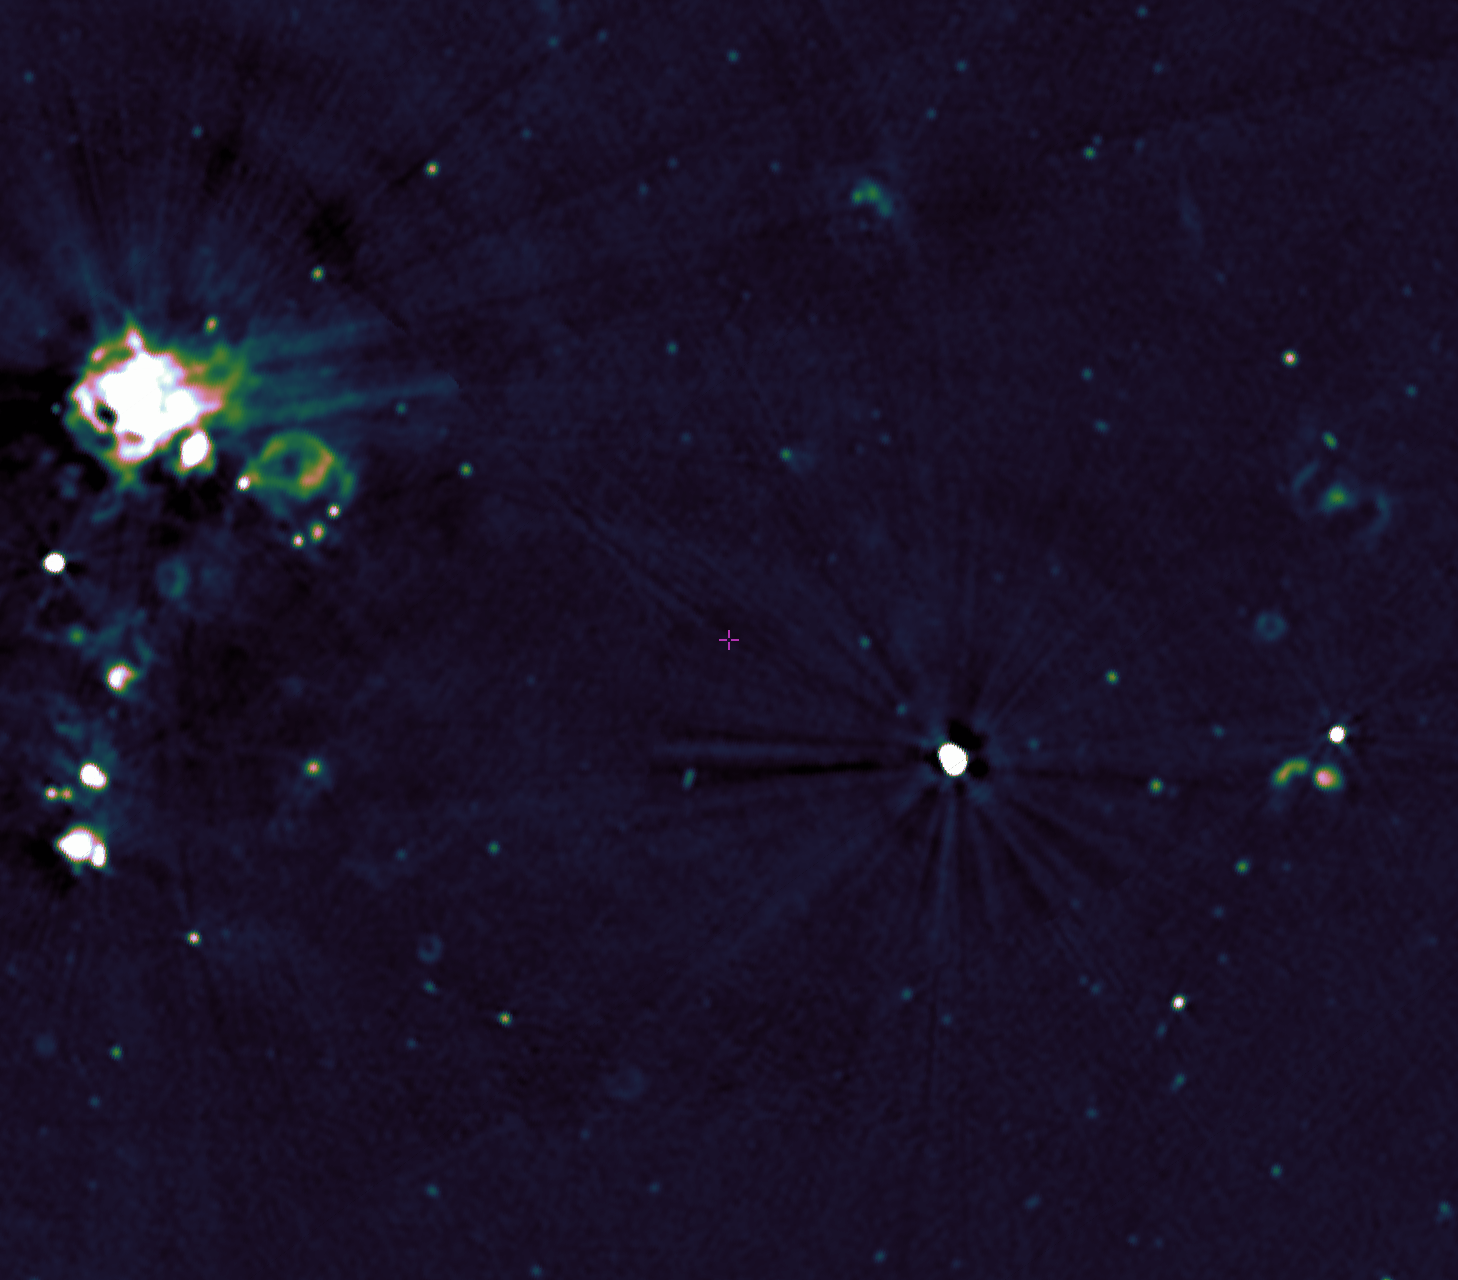
\includegraphics[width=1.0\linewidth]{./chapters/10.results/LMC/radio-843_cut.png}
		\caption{Radio wavelength at 843MHz.}
		\label{results:LMC:radio}
	\end{subfigure}
	\begin{subfigure}[b]{0.375\linewidth}
		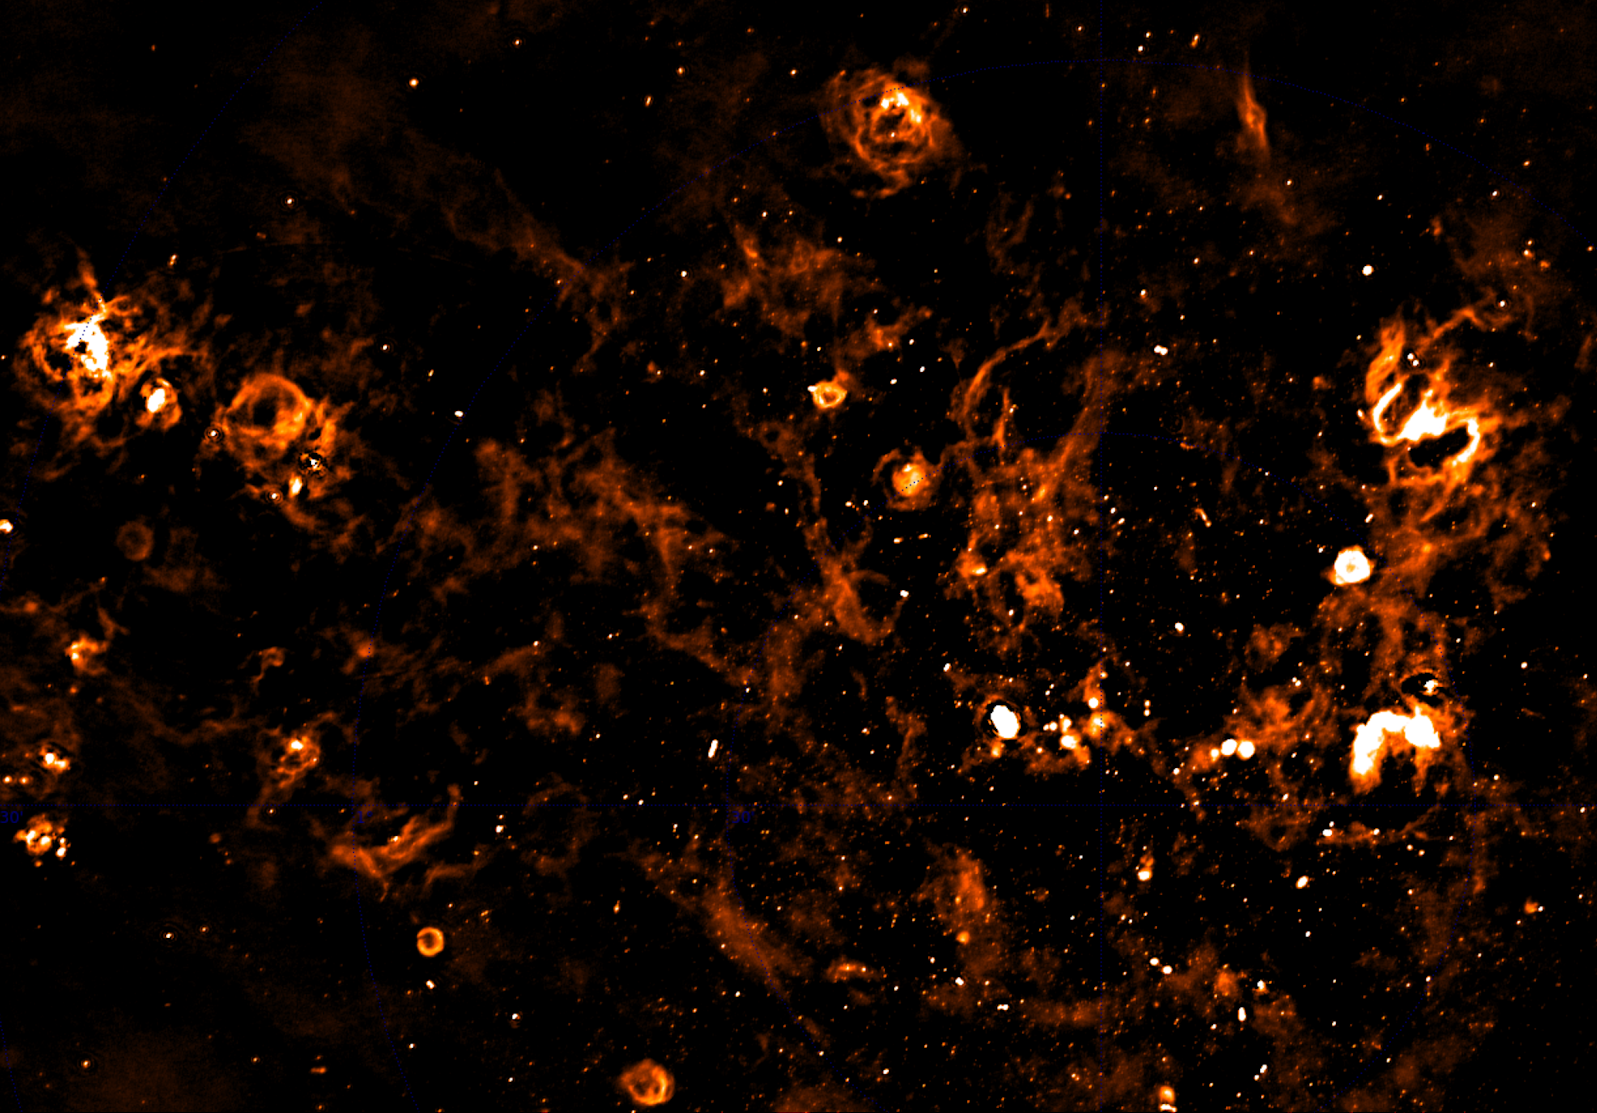
\includegraphics[width=1.0\linewidth]{./chapters/10.results/LMC/meerkat2.png}
		\caption{Wide band radio image by MeerKAT.}
		\label{results:LMC:meerkat}
	\end{subfigure}
	\caption{Section of the Large Magellanic Cloud (LMC)}
	\label{results:LMC}
\end{figure}

The MeerKAT observation covers a wide band of radio frequencies. The lowest frequency in the MeerKAT observation is 894 MHz, and the highest frequency is 1658 Mhz.
Imaging the whole frequency band requires a wide band deconvolution algorithm. In wide band imaging, several images at different frequencies get deconvolved as an image cube. Wide band imaging again multiplies the amount of work that has to be done for reconstruction, as now we cannot deconvolve a single image, but have to deal with a whole image cube.

Wide band imaging is not possible within the time frame of this project. We take a narrow band subset of 5 channels from the original data (ranging from 1084 to 1088 MHz, about 1 Gb in size) for reconstruction. We also reduce the field-of-view to a more manageable section. Figure \ref{results:cutout} shows the LMC image section we are using together with a CLEAN reconstruction of the narrow band data.

\begin{figure}[h]
	\centering
	\begin{subfigure}[b]{0.4\linewidth}
		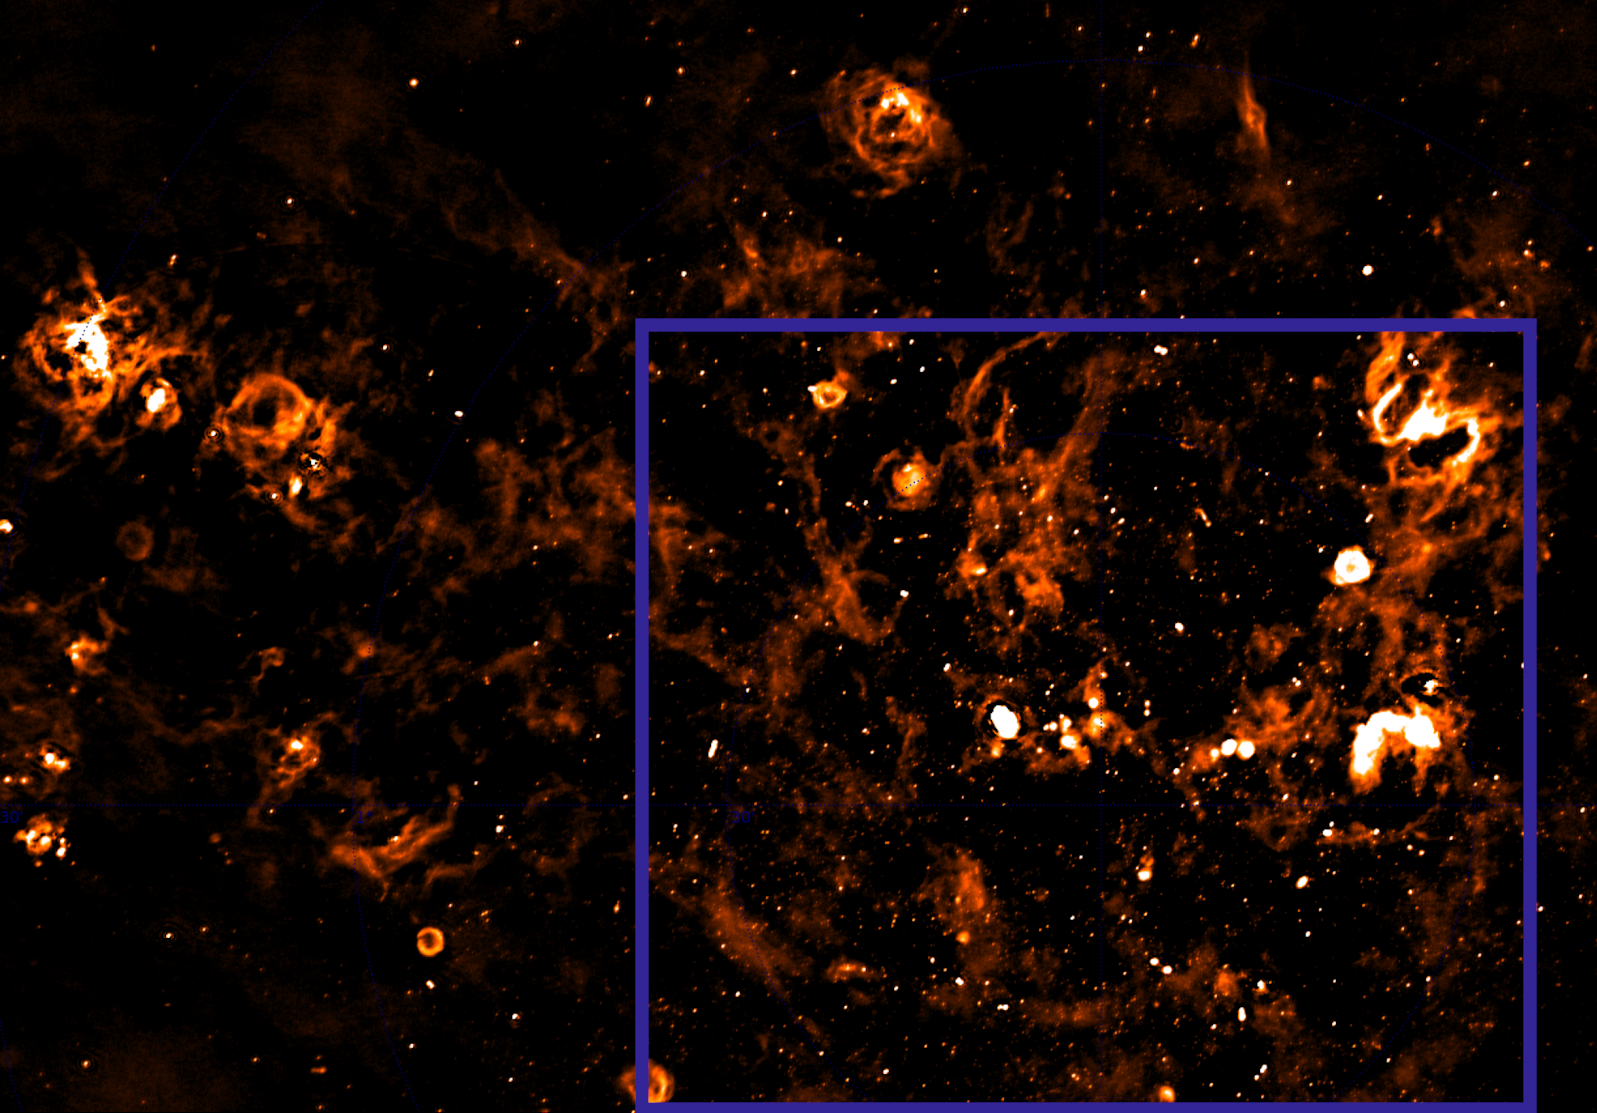
\includegraphics[width=1.0\linewidth]{./chapters/10.results/LMC/meerkat_cutout.png}
	\end{subfigure}
	\begin{subfigure}[b]{0.28\linewidth}
		\adjincludegraphics[width=1.0\linewidth, clip, trim={0.72in 0.72in 0.72in 0.72in}]{./chapters/10.results/MSClean/Briggs-CLEAN.png}
	\end{subfigure}
	\caption{Narrow band image section used.}
	\label{results:cutout}
\end{figure}

At the center of our image section \ref{results:cutout} we see the N132D supernova remnant. We partially see the faint extended emissions, although they are close to the noise level. This is known as a high-dynamic range reconstruction. We have strong radio sources mixed together with faint emissions, which are only marginally above the noise level of the image.

The total field-of-view of our image section is roughly 1.3 degrees(or 4600 arc seconds). Our reconstruction has $3072^2$ pixel with a resolution of 1.5 arc seconds per pixel. this is still a wide field-of-view reconstruction problem. We have to account for the effects of the $w$-term to achieve a high-dynamic range reconstruction.

In our test reconstruction, we need to account for $w$-term correction and high-dynamic range. We have excluded wide-band imaging as not feasible within the time frame of this project. In Section \ref{results:cleancomp} we compare the reconstructions of CLEAN with our serial coordinate descent algorithm on the LMC observation. The next Section \ref{results:speedup} presents the speedup we achieve with serial coordinate descent by using our distributed or GPU-accelerated implementations.

In Section \ref{results:gradients} we show the core result of this project. Namely what effect has an approximate $PSF$ on the deconvolution problem and whether we can use it to further distribute the problem. The answer to that question is affirmative: We can approximate the $PSF$, and we can exploit it to further distribute the deconvolution. But we need more sophisticated coordinate descent algorithms to fully benefit from it.


\subsection{Comparison with CLEAN reconstructions} \label{results:cleancomp}
We use the WSCLEAN \cite{offringa2014wsclean} implementation of multi-scale CLEAN algorithm. We compare our coordinate descent reconstruction with two CLEAN reconstructions, oe with naturally weighted visibilities and one with briggs-weighted visibilities.

There are three main visibility weighting scheme for the gridder that lead to different $PSF$s from the same measurements: Natural, uniform, and Briggs\cite{briggsWeighting}. Natural weighting scheme leads to an image with a lower noise level, but a wider $PSF$. Uniform weighting leads to a higher noise level, but to a $PSF$ which is more concentrated around a single pixel. Briggs weighting is a scheme combines the best from both worlds, receiving an image with acceptable noise level while getting a more concentrated $PSF$. As such it is widely used in radio astronomy image reconstruction. Our gridder implements the natural weighting scheme only. Nevertheless our coordinate descent algorithm is able to retrieve structures similar to the briggs-weighted multi-scale CLEAN reconstruction, even though coordinate descent has to work with a wider $PSF$.

Figure \ref{results:cleancomp:figure} shows the reconstruction of both briggs-weighted multi-scale CLEAN and the naturally weighted coordinate descent reconstruction. We used a regularization parameter of $\lambda = 1.0 * Lipschitz$ and $\alpha = 0.01$. The elastic net regularization is biased heavily towards the L2 norm. We stopped the serial coordinate descent if every possible pixel change is below $\epsilon = 1e^{-5}$. We use these parameters for the whole project unless we specify otherwise.

\newpage

\begin{figure}[h]
	\centering
	\begin{subfigure}[b]{0.49\linewidth}
		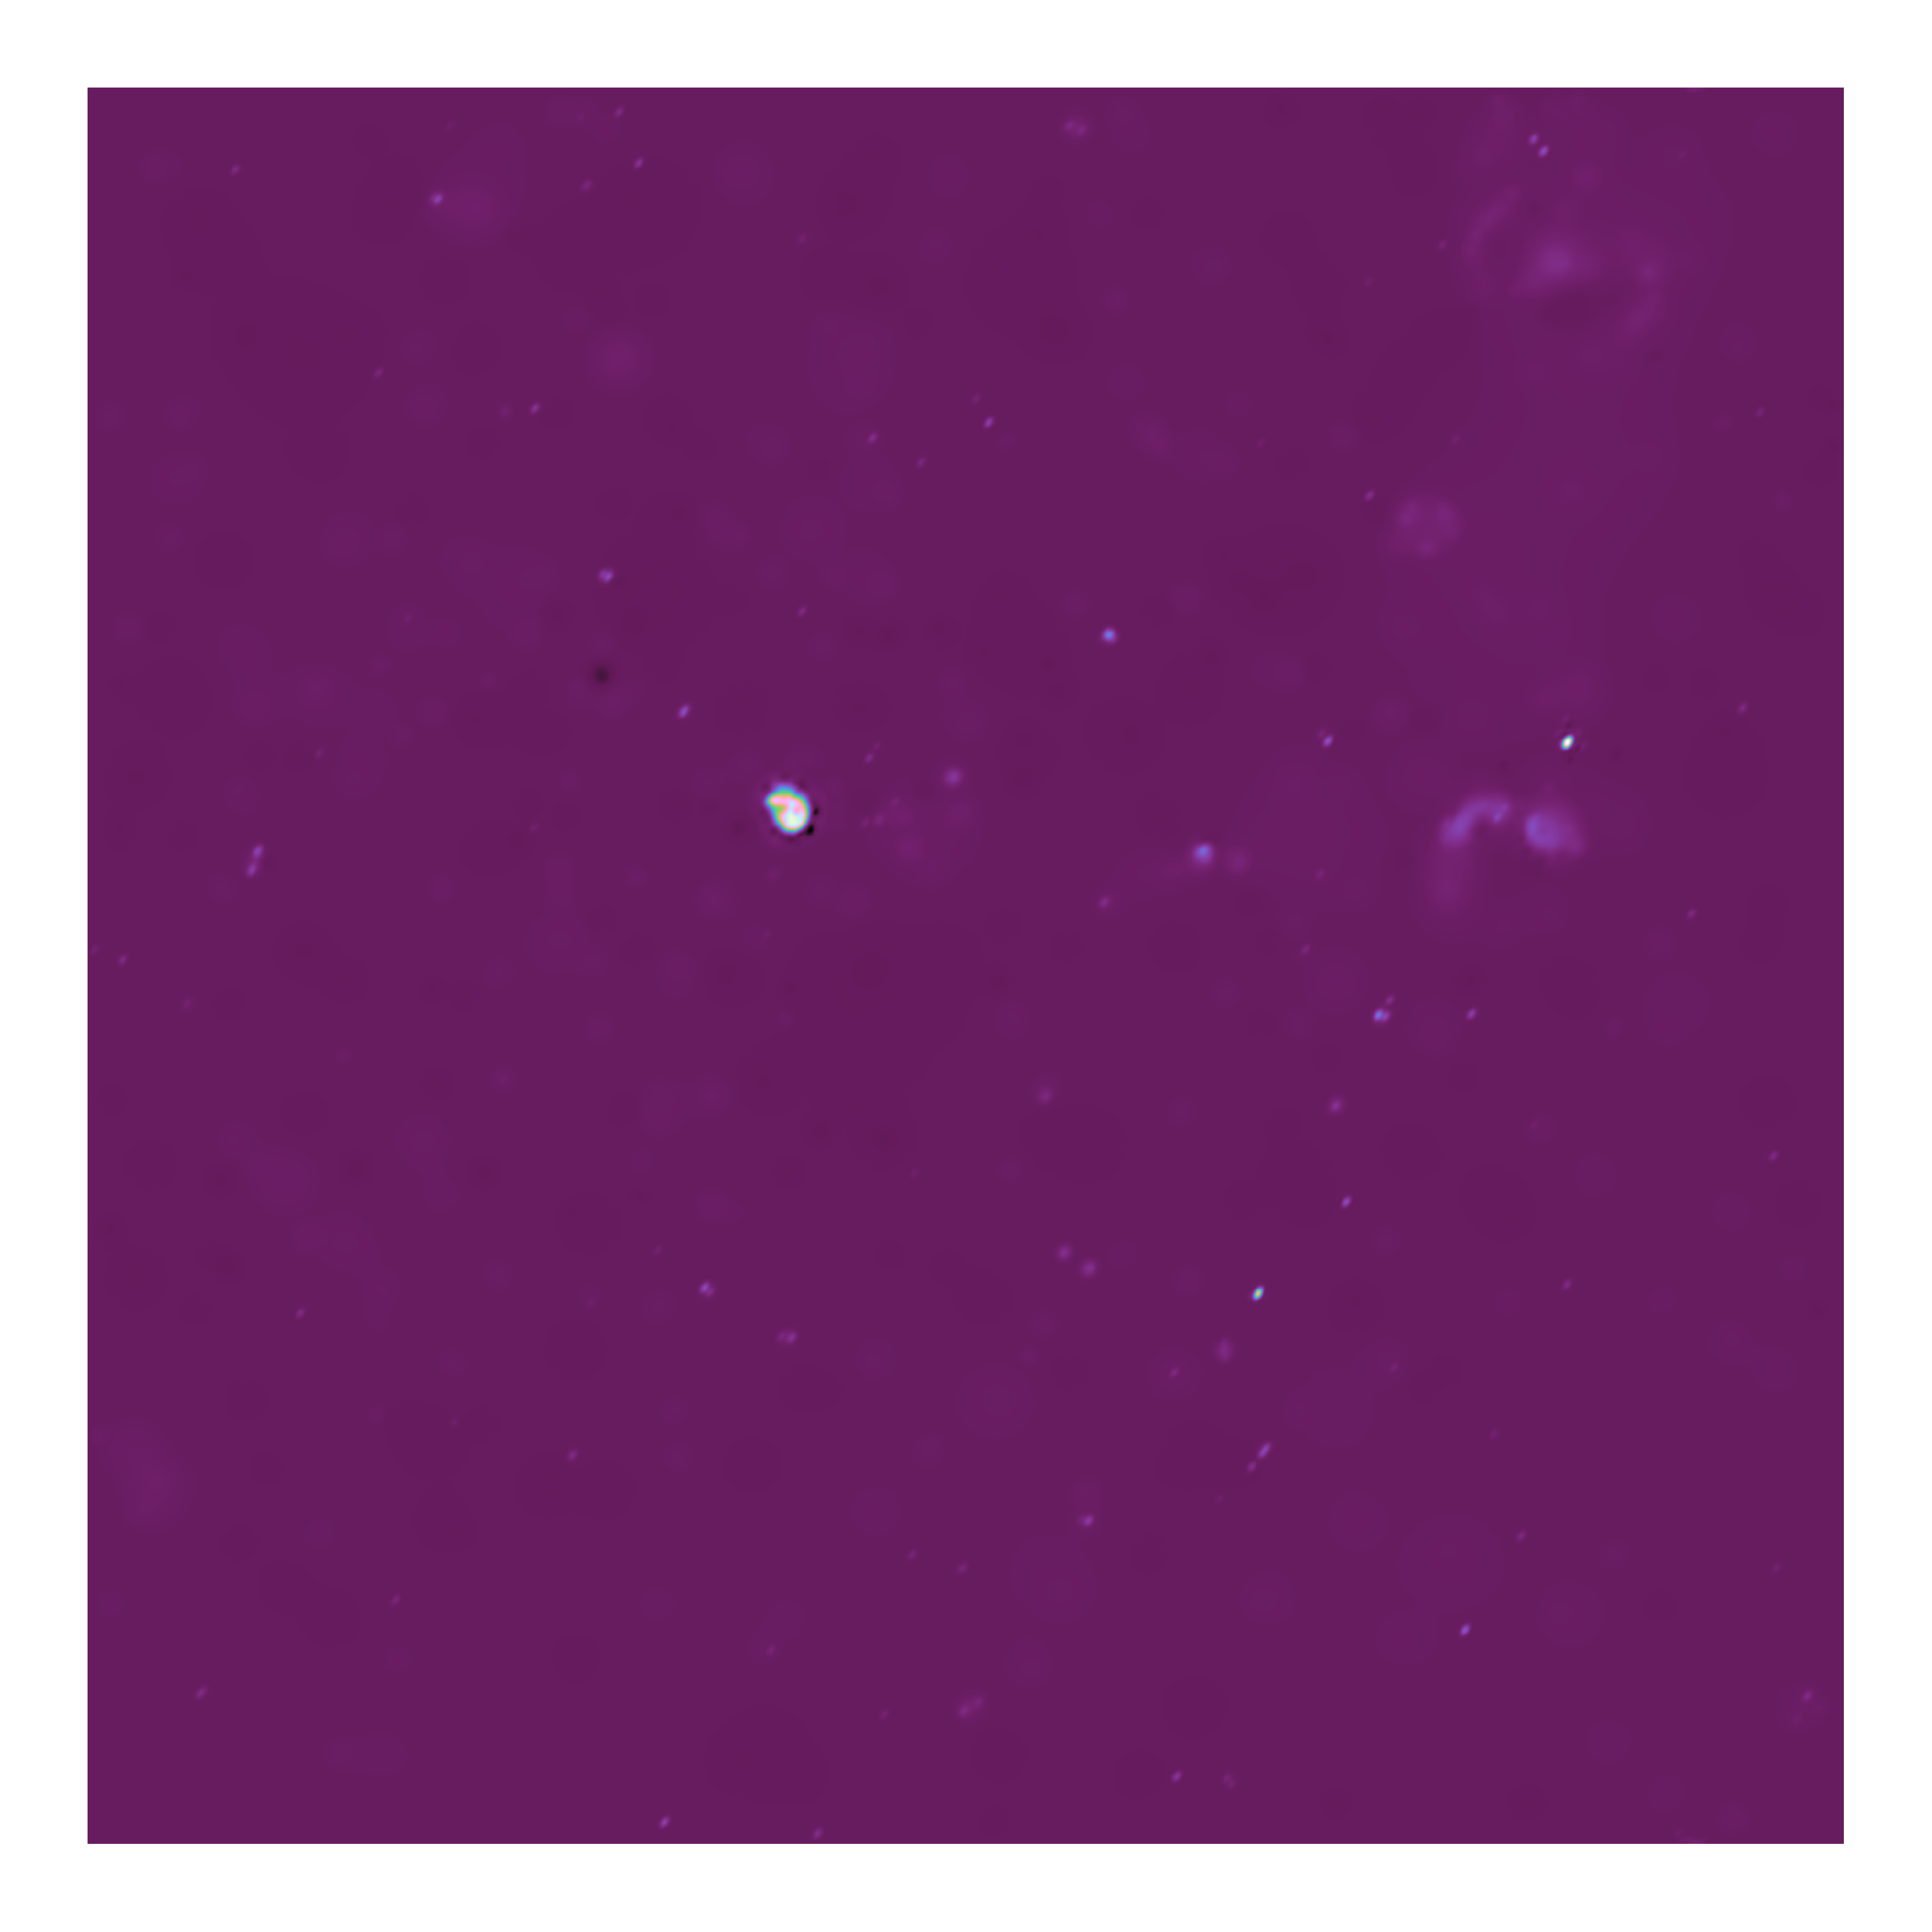
\includegraphics[width=1.00\linewidth, clip, trim={0.72in 0.72in 0.72in 0.72in}]{./chapters/10.results/MSClean/Briggs-CLEAN.png}
		\caption{Briggs weighted multi-scale CLEAN.}
		\label{results:comp:clean}
	\end{subfigure}
	\begin{subfigure}[b]{0.49\linewidth}
		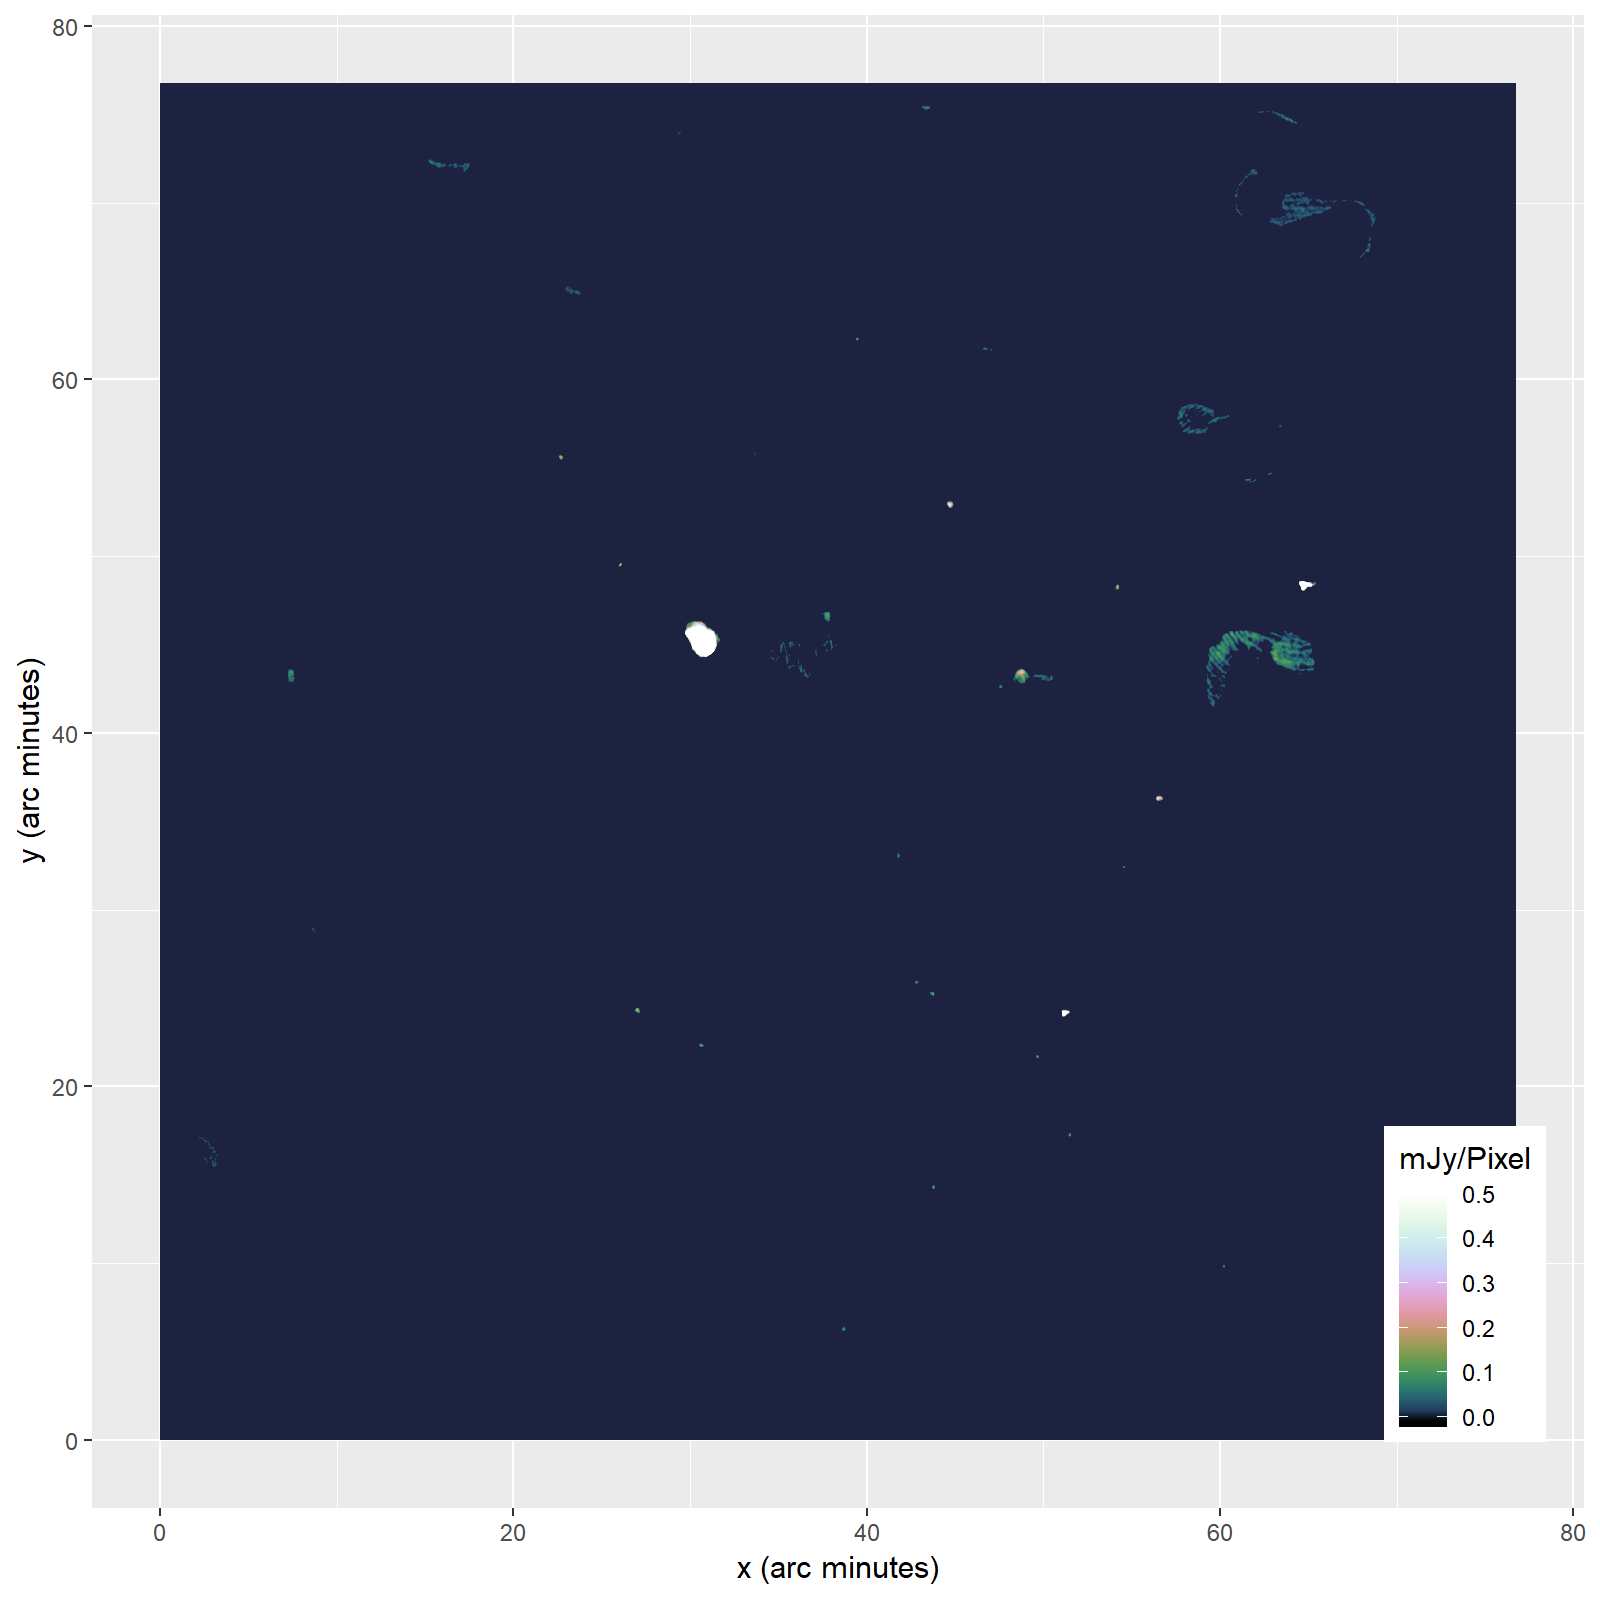
\includegraphics[width=1.00\linewidth, clip, trim={0.72in 0.72in 0.72in 0.72in}]{./chapters/10.results/SerialCD/CD-reference.png}
		\caption{Naturally weighted coordinate descent.}
		\label{results:comp:cd}
	\end{subfigure}
	\\
	\begin{subfigure}[b]{0.49\linewidth}
		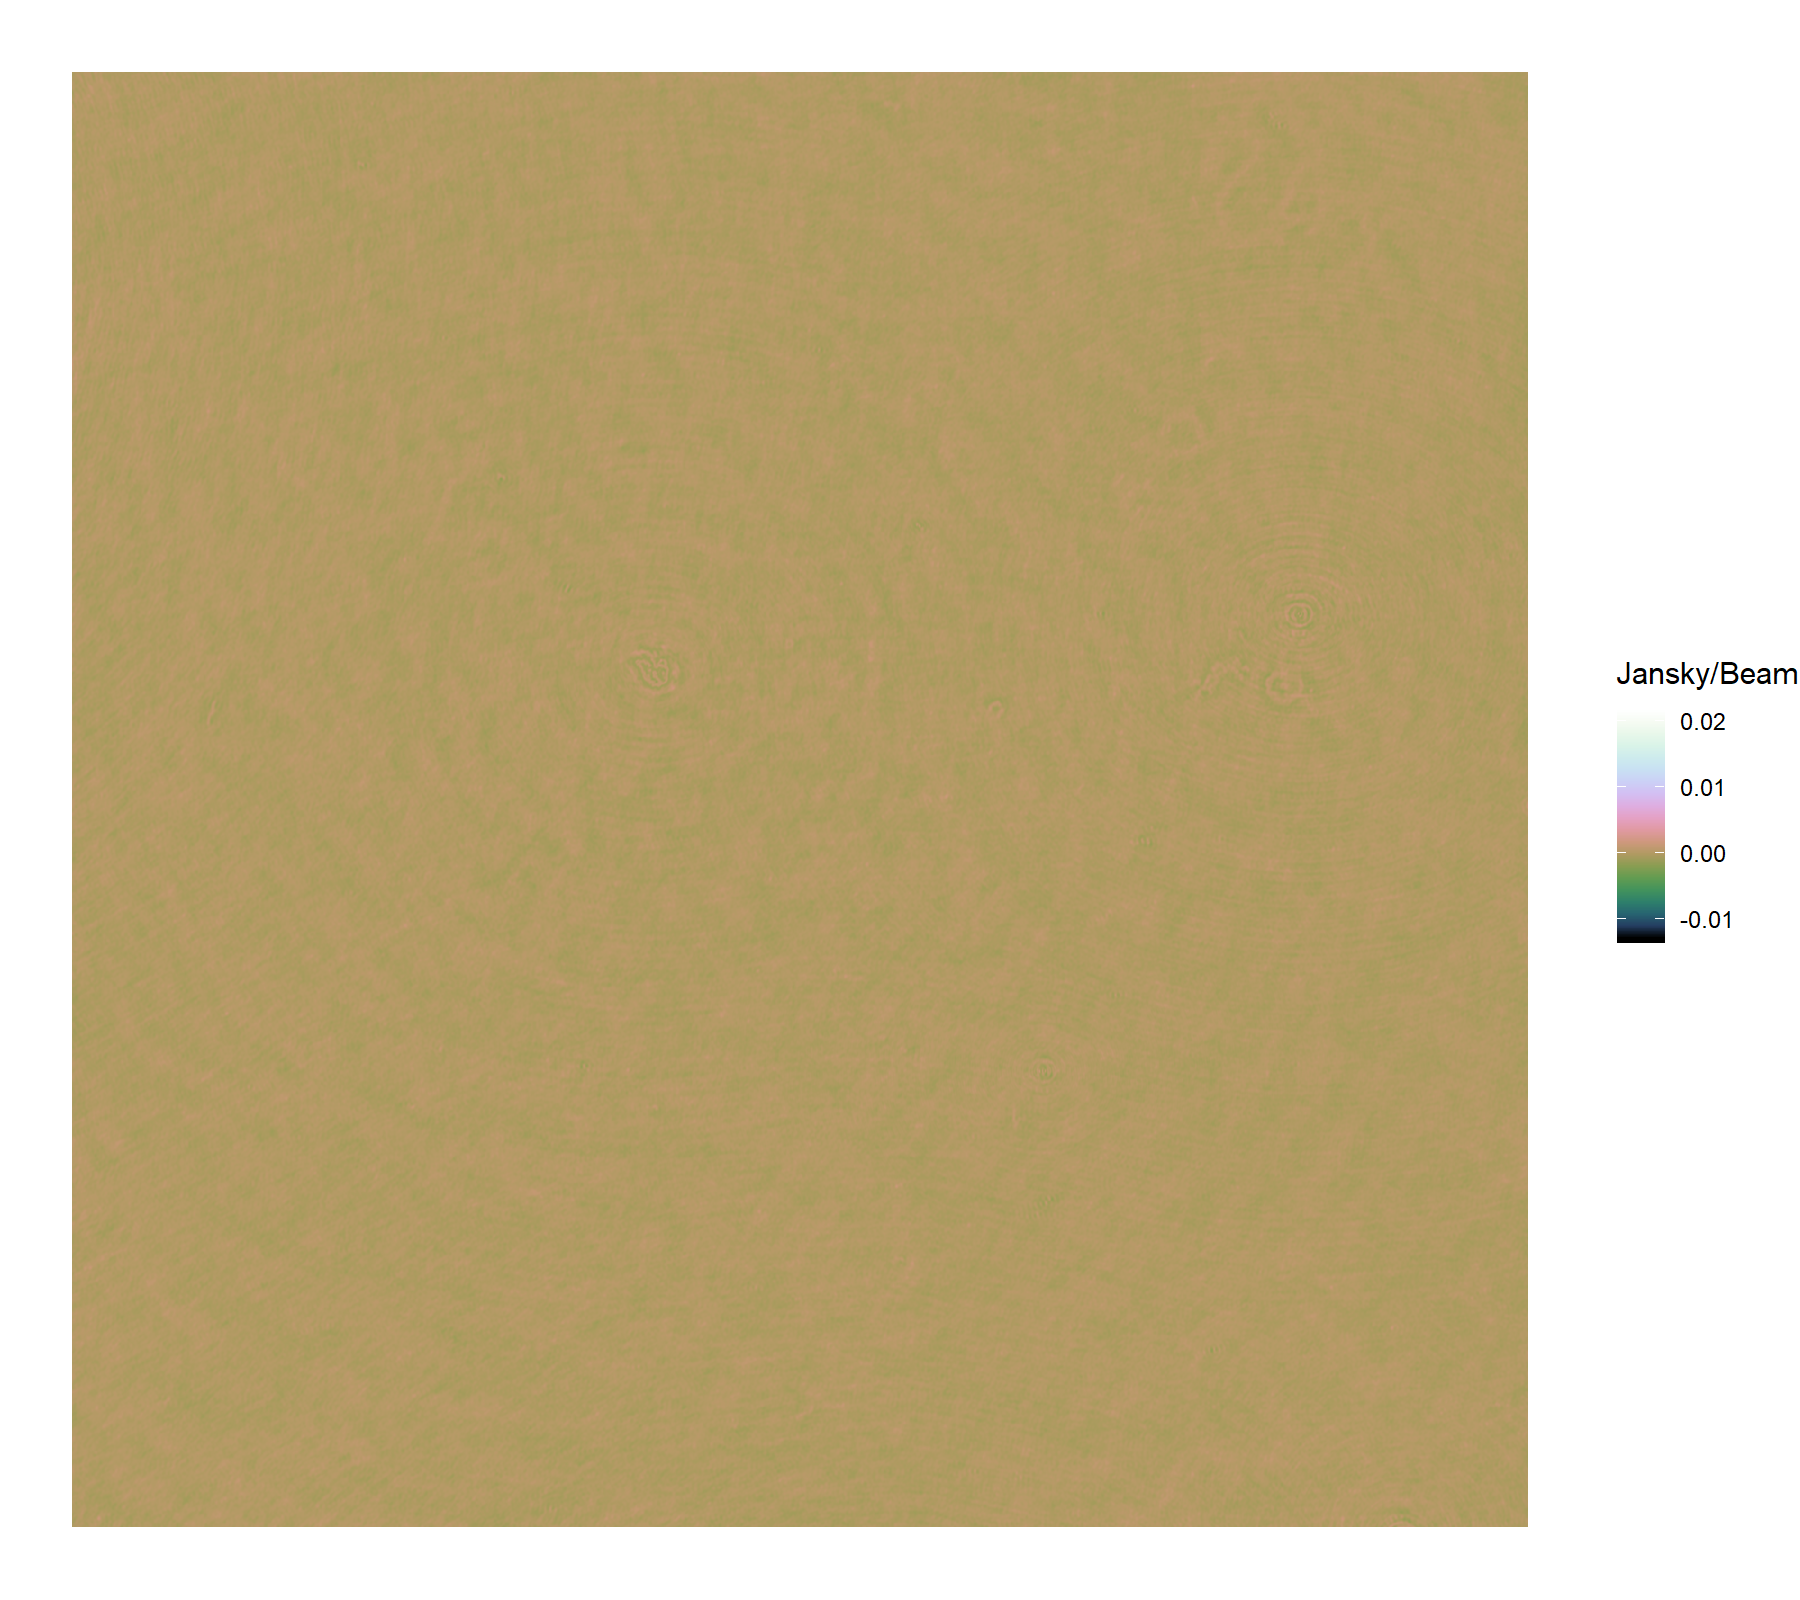
\includegraphics[width=1.00\linewidth, clip, trim={0.36in 0.36in 0.0in 0.36in}]{./chapters/10.results/MSClean/briggs-CLEAN-residuals.png}
		\caption{Residuals of multi-scale CLEAN.}
		\label{results:comp:clean-res}
	\end{subfigure}
	\begin{subfigure}[b]{0.49\linewidth}
		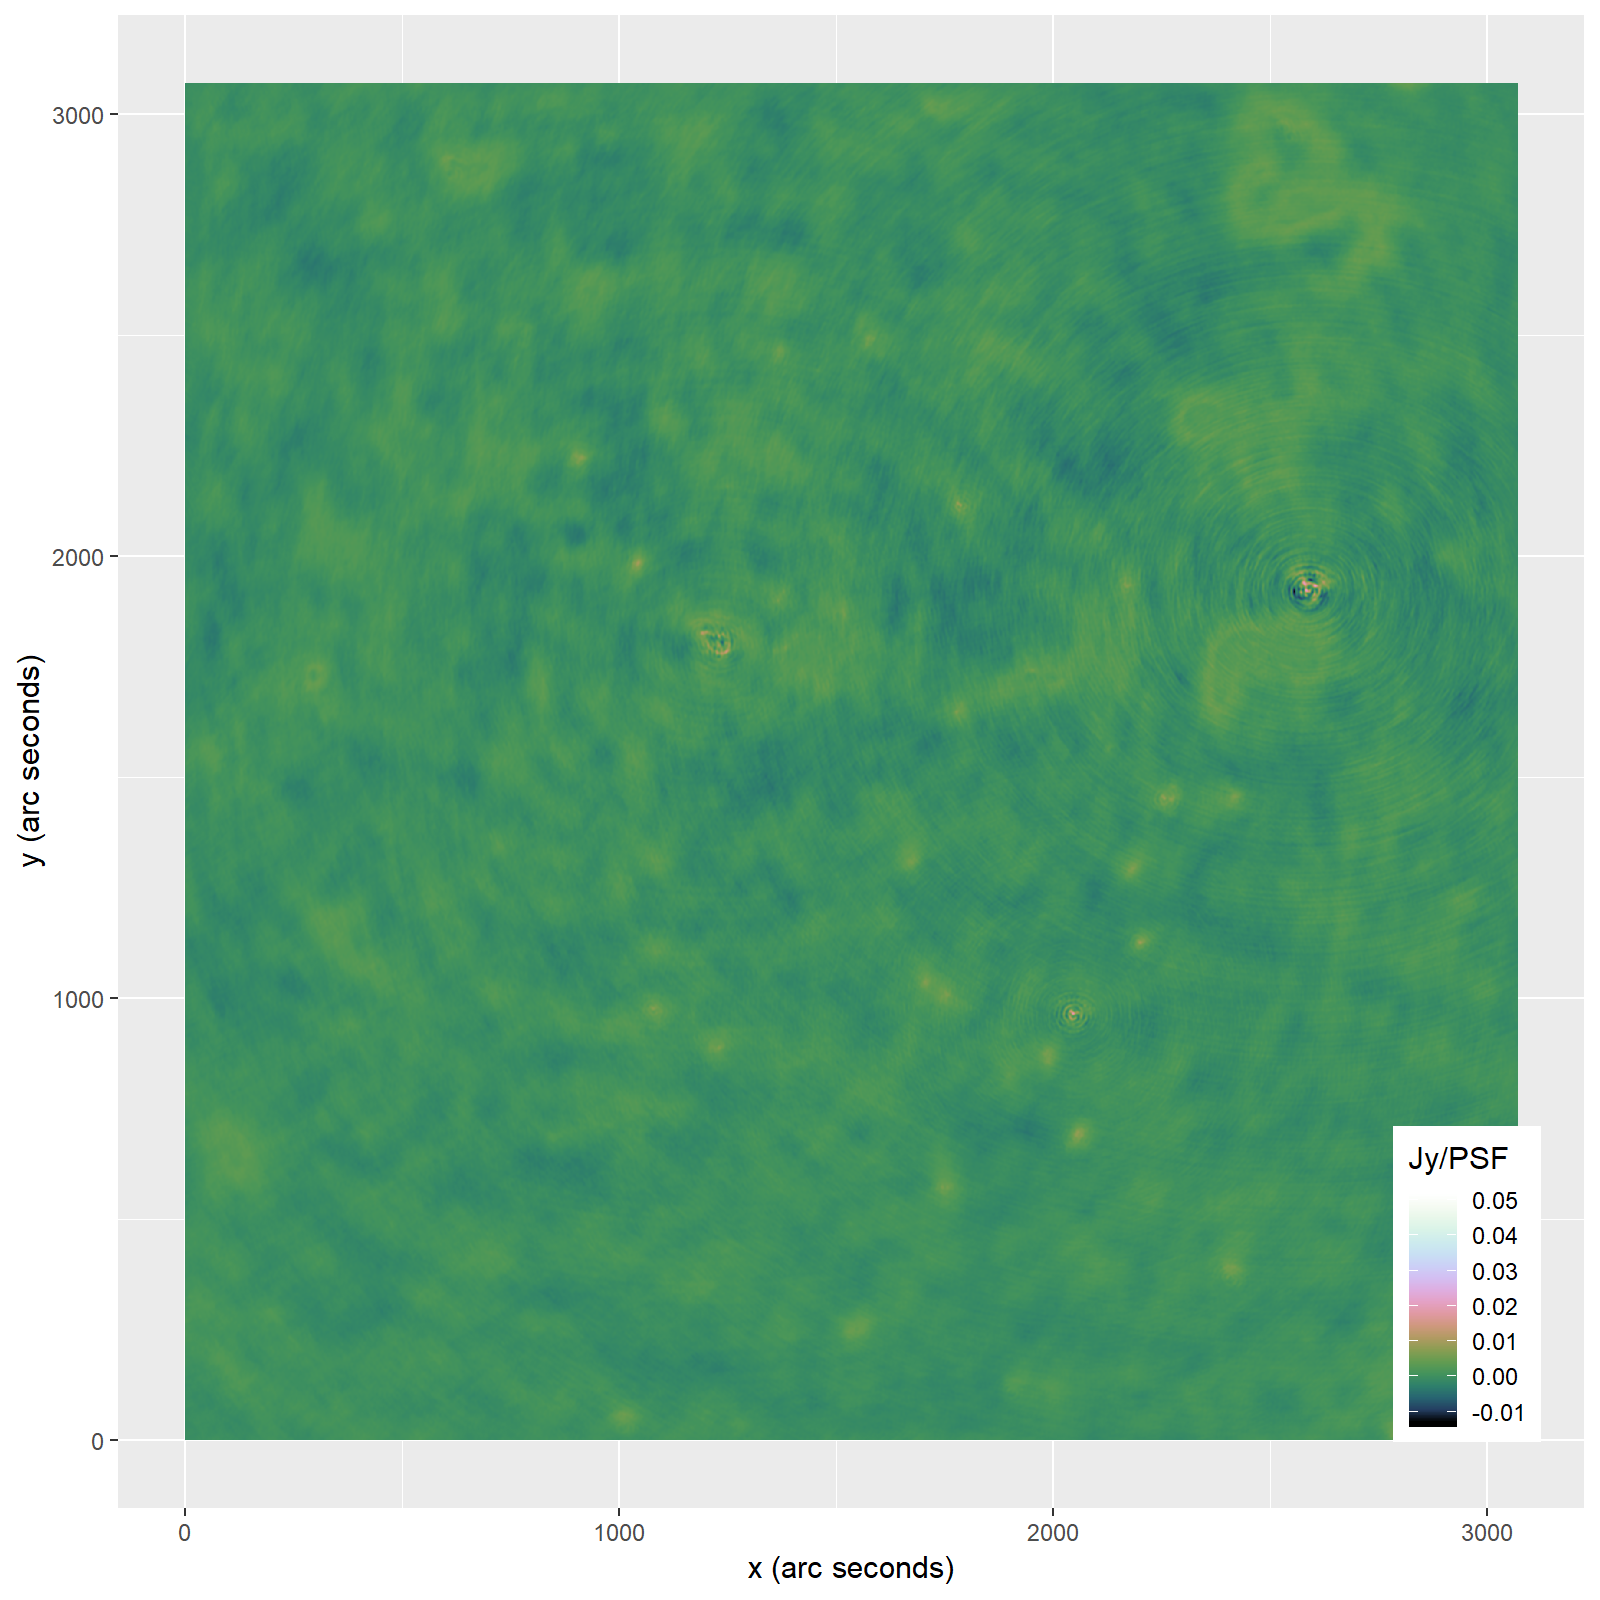
\includegraphics[width=1.00\linewidth, clip, trim={0.36in 0.36in 0.0in 0.36in}]{./chapters/10.results/SerialCD/CD-reference-residuals.png}
		\caption{Residuals of coordinate descent.}
		\label{results:comp:cd-res}
	\end{subfigure}

	\caption{Comparison of the whole image}
	\label{results:cleancomp:figure}
\end{figure}

\newpage

Multi-scale reconstructed its image within 6 Major and 14 thousand Minor cycle iterations. Our serial coordinate descent algorithm converged after 5 Major cycles and used 100 thousand iterations to converge. Our algorithm required roughly 8 times more iterations. It took a total of 35 minutes to reconstruct an image on an Intel Xeon E3-1505M with 8 logical cores. On this data set, our algorithm used one Major cycle less than multi-scale CLEAN. However, the number of Major cycles is not directly comparable. We do not use the identical criteria to initiate another Major cycle: At the beginning of each deconvolution, we check the maximum pixel difference. If it is below $\epsilon_{major} = 1e^{-4}$, we stop the reconstruction. We have not compared our stopping criterion to WSCLEAN. As such, the number of Major cycles are only a rough comparison. Our serial coordinate descent uses a similar number of Major cycles as multi-scale CLEAN.

Both algorithms detect the three extended emissions at the right side of the image. They detect various point sources at the same location. Coordinate descent and multi-scale CLEAN arrive at a roughly similar result. Coordinate descent detects similar structures in the N132D supernova remnant, as the briggs-weighted CLEAN, but also includes calibration errors in its reconstruction of the faint extended emissions.

When we compare the reconstruction quality of multi-scale CLEAN an our serial coordinate descent algorithm, we note that the magnitudes of the residual image of multi-scale CLEAN \ref{results:comp:clean-res} is significantly lower than the magnitudes in our algorithm, shown in \ref{results:comp:cd-res}. In the residual image of the serial coordinate descent algorithm, we still see some emissions belonging to stars, or extended emissions. This is to be expected, as multi-scale CLEAN uses several heuristics developed specifically for radio interferometric imaging\cite{offringa2017optimized}. Note however that the serial coordinate descent algorithm leaves large negative values in the residual image, while multi-scale CLEAN includes it in its reconstruction. Multi-scale CLEAN has several areas of negative pixel values, which is implausible.


\begin{figure}[h]
	\centering
	\begin{subfigure}[b]{0.32\linewidth}
		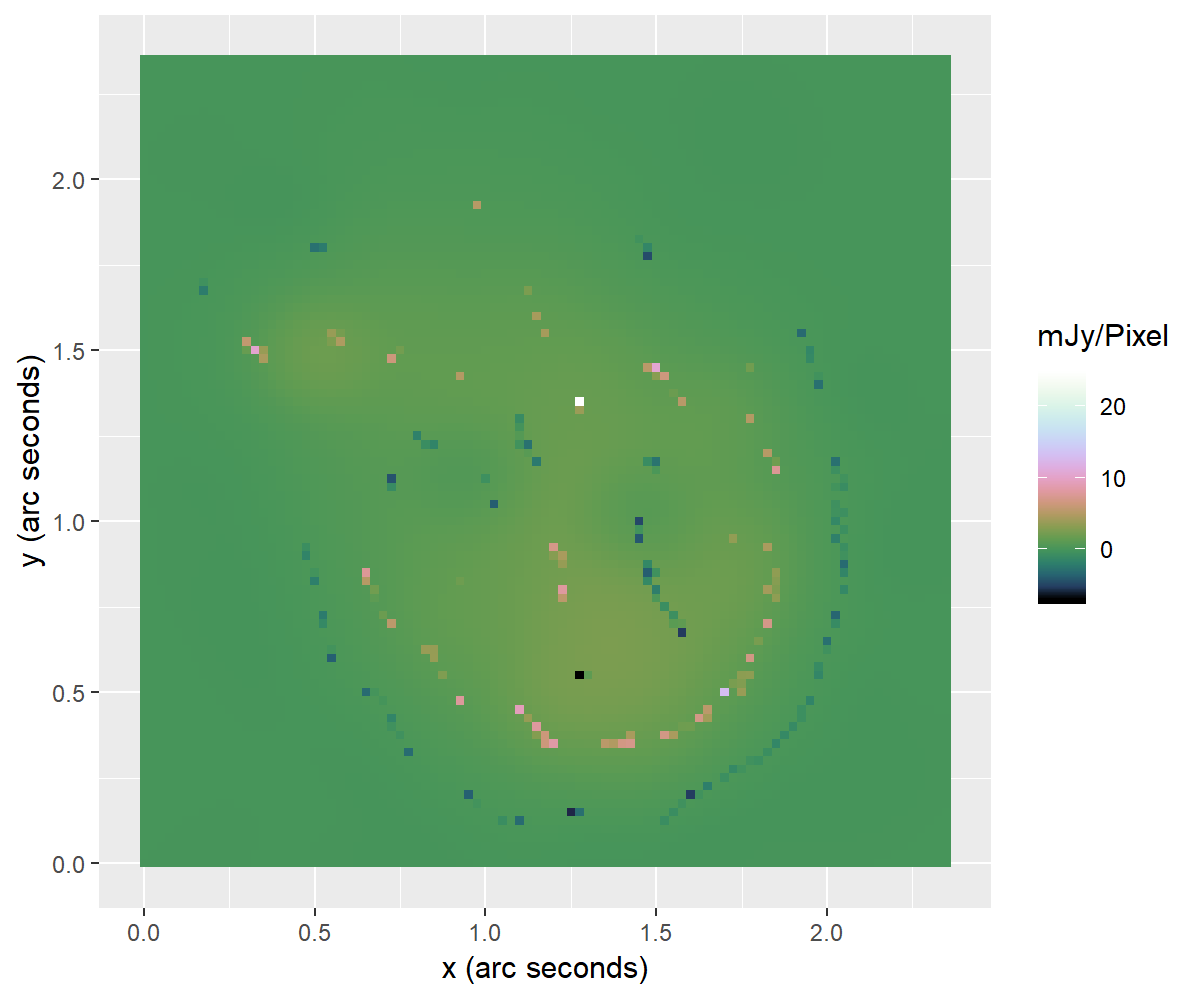
\includegraphics[width=1.00\linewidth]{./chapters/10.results/MSClean/Natural-N132.png}
		\caption{CLEAN Natural weighting.}
		\label{results:N132:clean}
	\end{subfigure}
	\begin{subfigure}[b]{0.32\linewidth}
		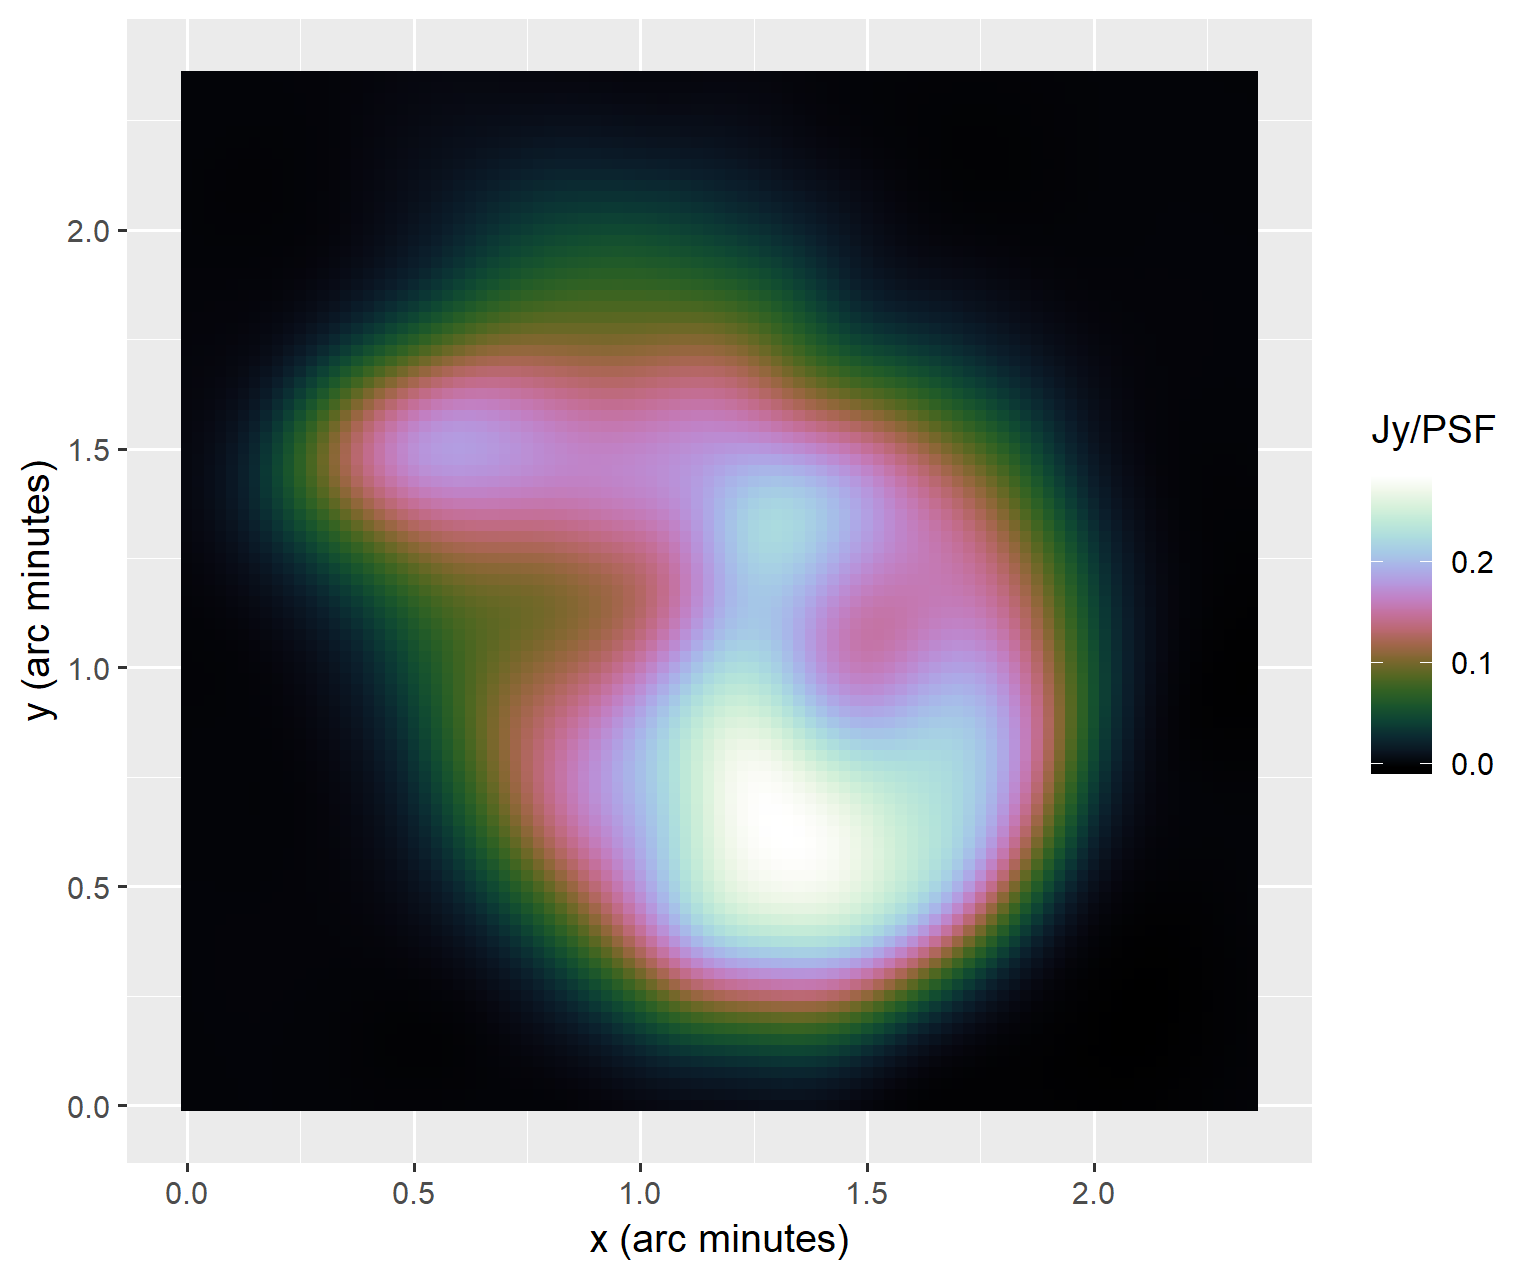
\includegraphics[width=1.00\linewidth]{./chapters/10.results/MSClean/Briggs-N132.png}
		\caption{CLEAN Briggs weighting.}
		\label{results:N132:cleanbriggs}
	\end{subfigure}
	\begin{subfigure}[b]{0.32\linewidth}
		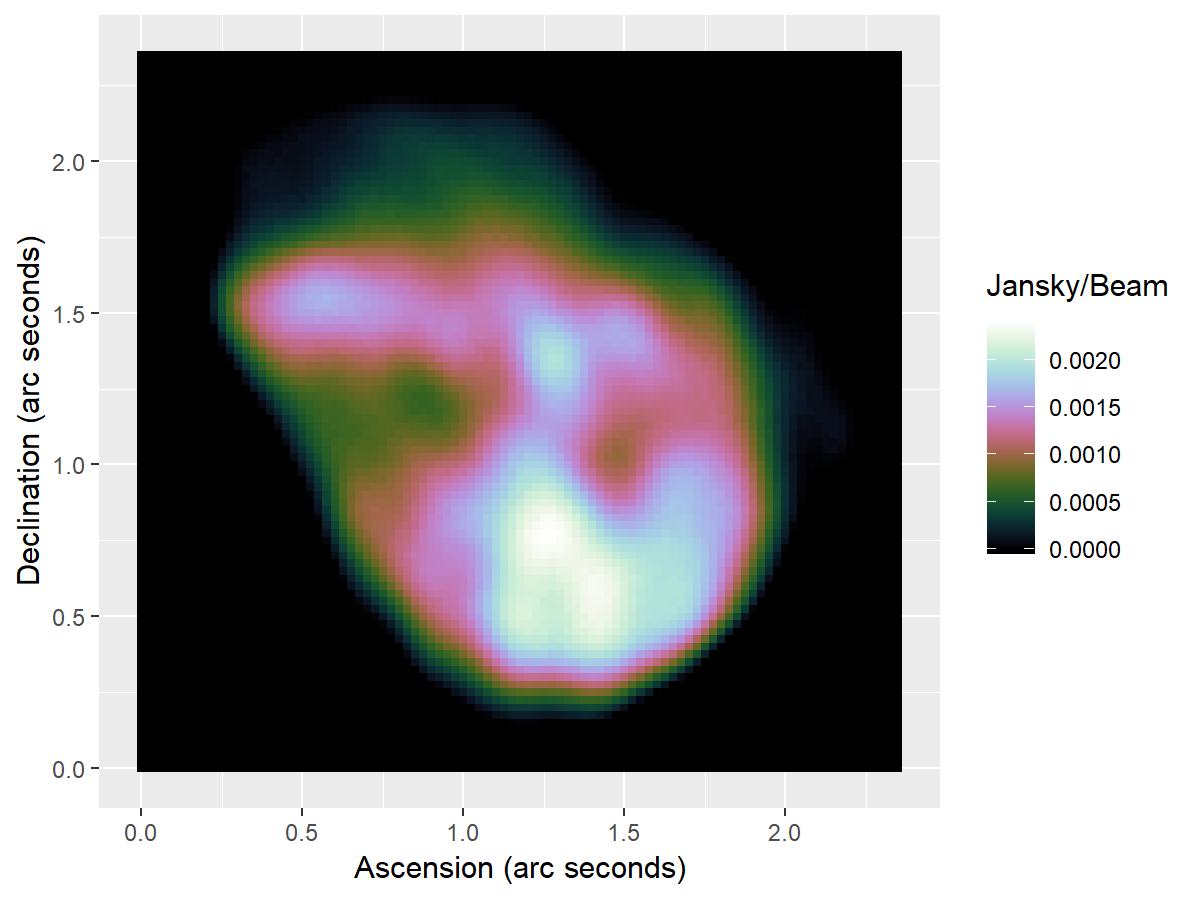
\includegraphics[width=1.00\linewidth]{./chapters/10.results/SerialCD/CD-N132.png}
		\caption{CD Natural weighting.}
		\label{results:comp:N132:cd}
	\end{subfigure}
	\caption{N132D comparison}
	\label{results:cleancomp::N132:figure}
\end{figure}

We now compare sections of the briggs-weighted multi-scale CLEAN with our naturally weighted serial coordinate descent algorithm. We compare the reconstruction of the N132D supernova-remnant in Figure \ref{results:cleancomp::N132:figure}. For comparison, we also included the naturally weighted mutli-scale CLEAN reconstruction in Figure \ref{results:N132:clean}. With natural weighting, multi-scale CLEAN reconstructs N132D as a Gaussian blob. Serial coordinate descent on the other hand is able to find structures inside the remnant with the same $PSF$, shown in Figure \ref{results:comp:N132:cd}. These are plausible super-resolved structures. They are also detected with briggs-weighted multi-scale CLEAN, shown in Figure \ref{results:N132:cleanbriggs}. But mutli-scale CLEAN needs briggs-weighting to reconstruct the smaller structures. As we mentioned, briggs-weighting leads to a more concentrated $PSF$.

\begin{figure}[h]
	\centering
	\begin{subfigure}[b]{0.45\linewidth}
		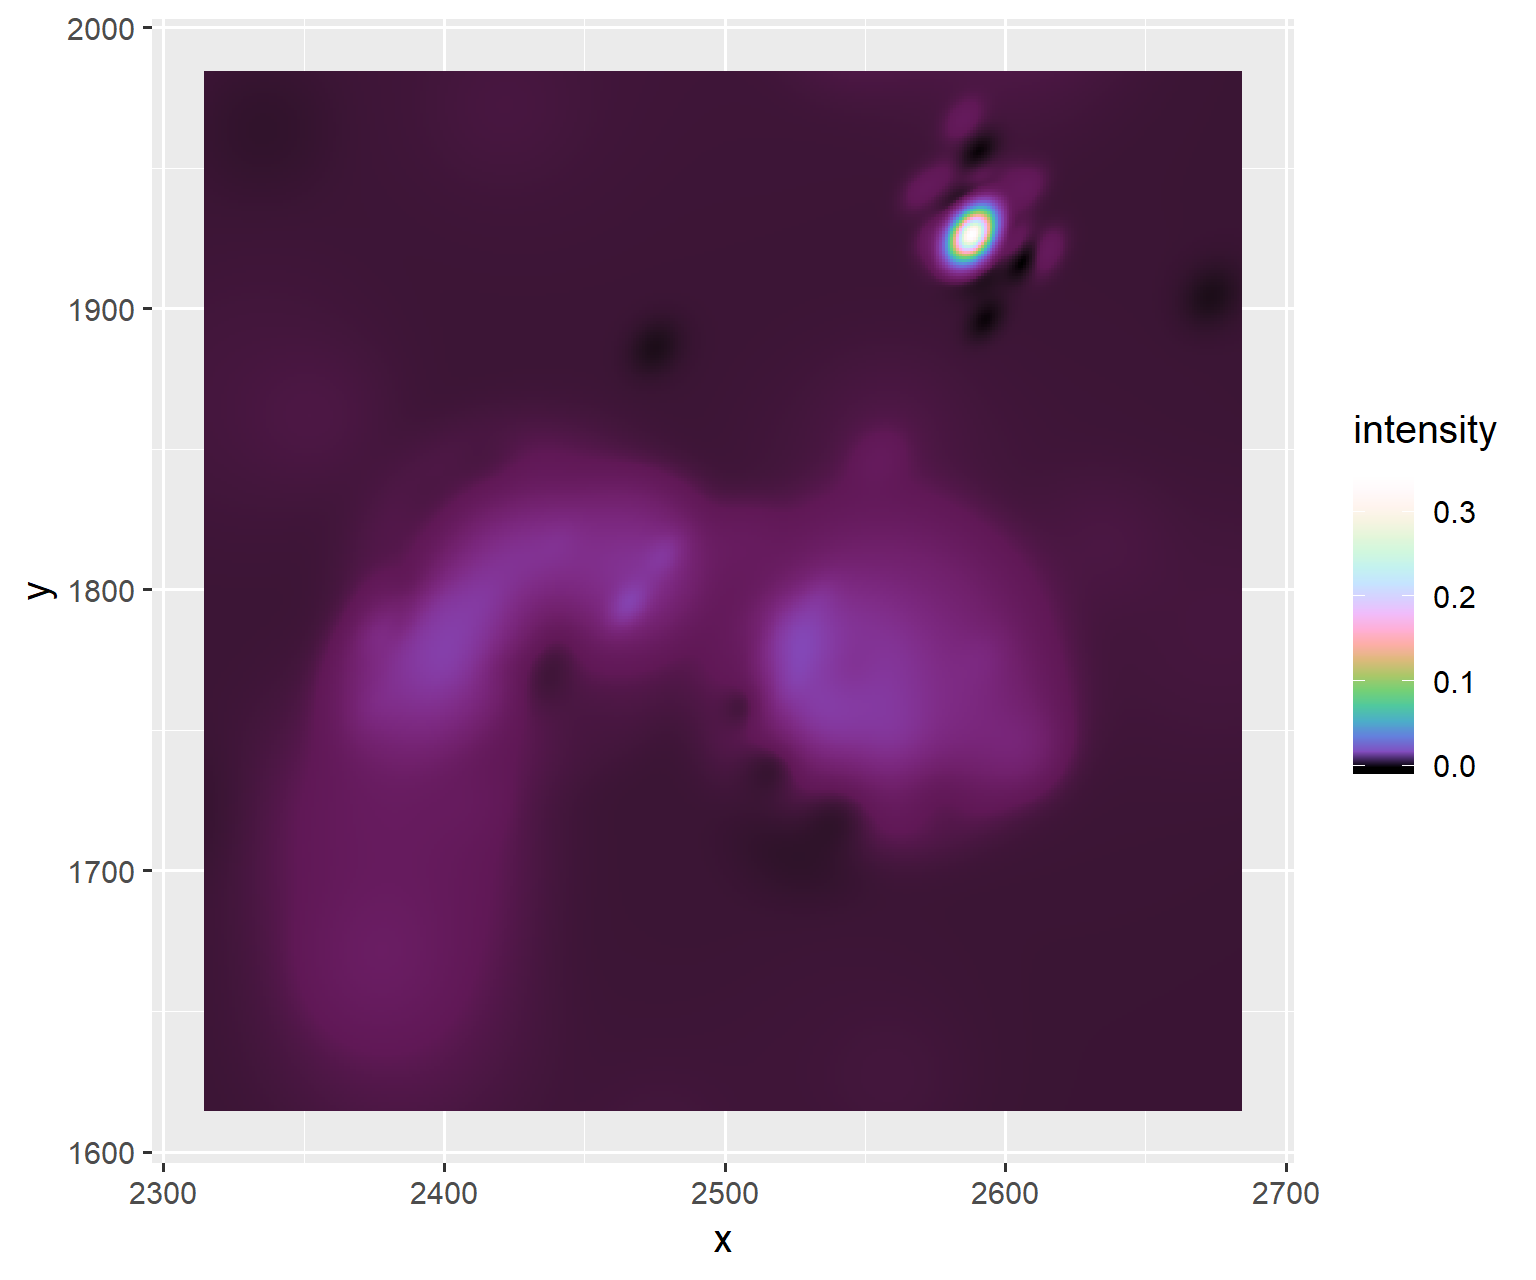
\includegraphics[width=1.00\linewidth]{./chapters/10.results/MSClean/Briggs-Calibration.png}
		\caption{Briggs CLEAN}
	\end{subfigure}
	\begin{subfigure}[b]{0.45\linewidth}
		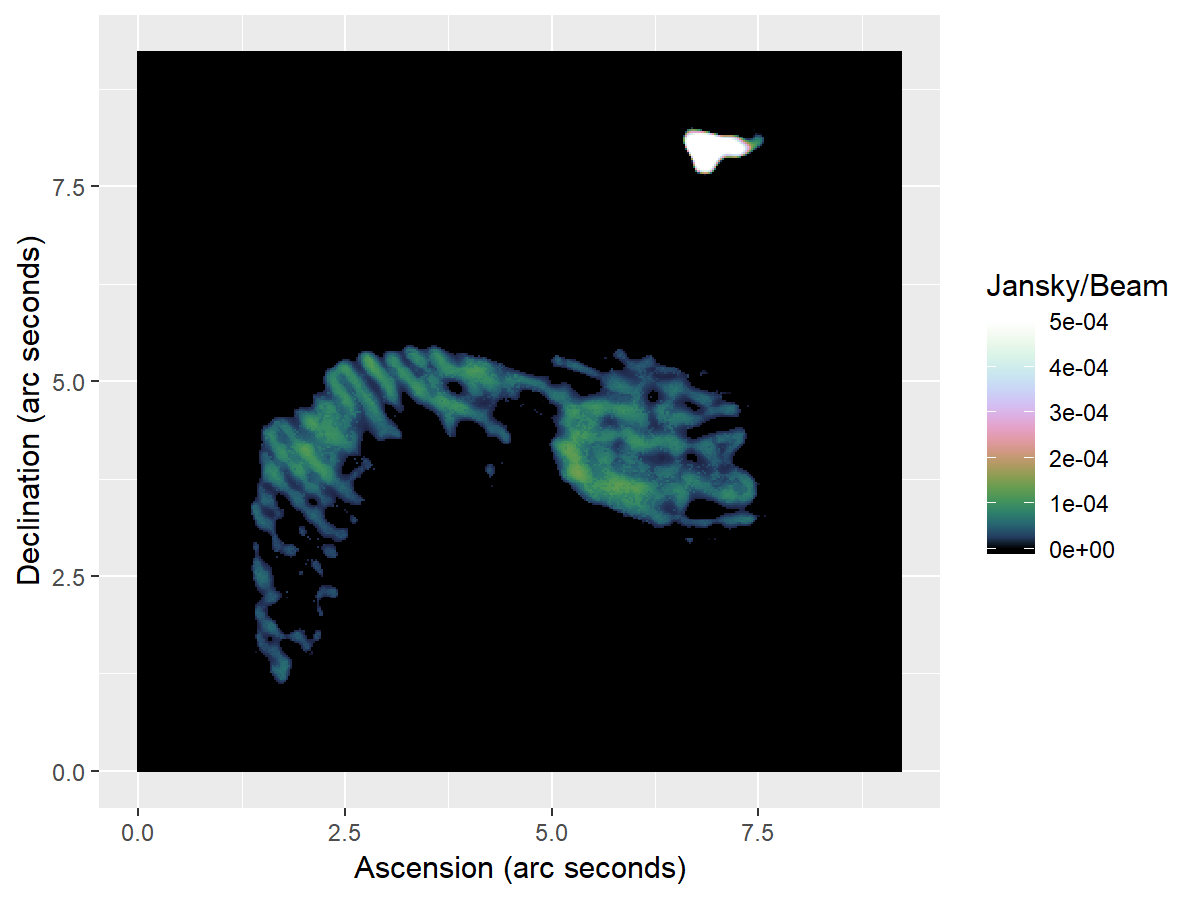
\includegraphics[width=1.00\linewidth]{./chapters/10.results/SerialCD/CD-Calibration.png}
		\caption{Coordinate Descent}
	\end{subfigure}
	\caption{Influence of calibration errors}
	\label{results:cleancomp::calib:figure}
\end{figure}

If we compare the reconstruction algorithm on areas with calibration errors, we clearly see that it negatively influences the reconstruction of serial coordinate descent. Figure \ref{results:cleancomp::calib:figure} shows a cutout of the right hand section of the reconstruction, where a faint extended emission is next to a point source with calibration errors. Multi-scale CLEAN is able to differentiate between the 'ripples' from the calibration error, and the extended emission. Coordinate descent with the elastic net regularization includes the ripples into the reconstructed image. 

The easiest way to exclude the calibration ripples from the reconstruction is to increase the regularization parameter $\lambda$, such as no pixel gets included which is not above the noise level + calibration error in the image. However, that would lead to other sources being "regularized away" in other regions of the image, which do not have a severe calibration error close by. 


\subsection{Serial coordinate descent speedup with MPI or GPU}\label{results:speedup}
In this section we test how much we can speed-up our serial coordinate descent algorithm by using distributed computing with MPI, or GPU acceleration.

We test the distributed serial coordinate descent on a shared memory system(Meaning all CPUs have access to the same main memory) with 32 CPUs. This is a best-case scenario for our implementation, because each node runs on the same physical machine: Our implementation needs a communication step between the nodes for each serial coordinate descent iteration. It needs a low-latency connection between each node to run as efficient as possible. Since each node runs on the same physical machine, it has a low latency times and therefore a low communication time. In this implementation, each node uses a single processor. We compare the speedup the algorithm achieves by adding more nodes/processors.

For the GPU we used personal computer level hardware, and tested on a nVidia Quadro M1200. We compare the speedup we achieve to the on-board CPU, which is an Intel Xeon E3-1505M with 8 logical processors at different image sizes. The speedup is shown in Figure \ref{results:speedup:figure}.

\begin{figure}[h]
	\centering
		\begin{subfigure}[b]{0.45\linewidth}
		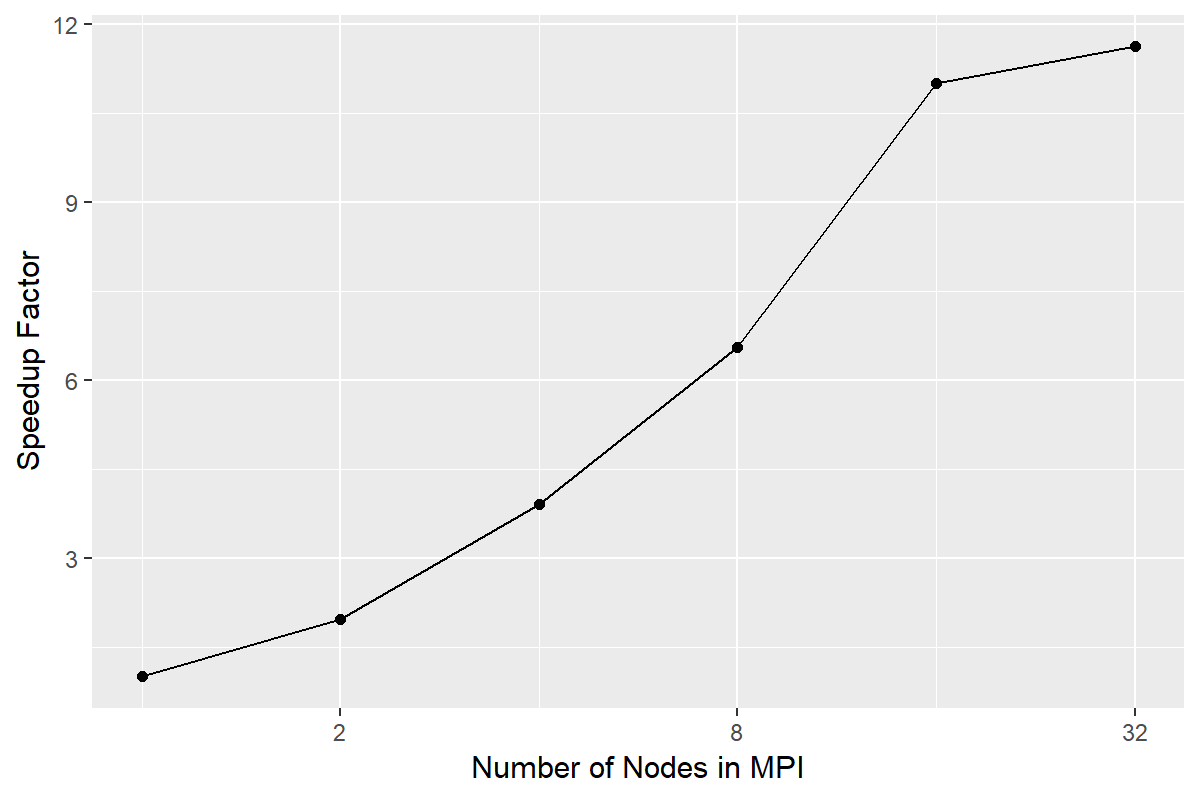
\includegraphics[width=1.00\linewidth]{./chapters/10.results/speedup/dist-speedup.png}
	\end{subfigure}
	\begin{subfigure}[b]{0.45\linewidth}
		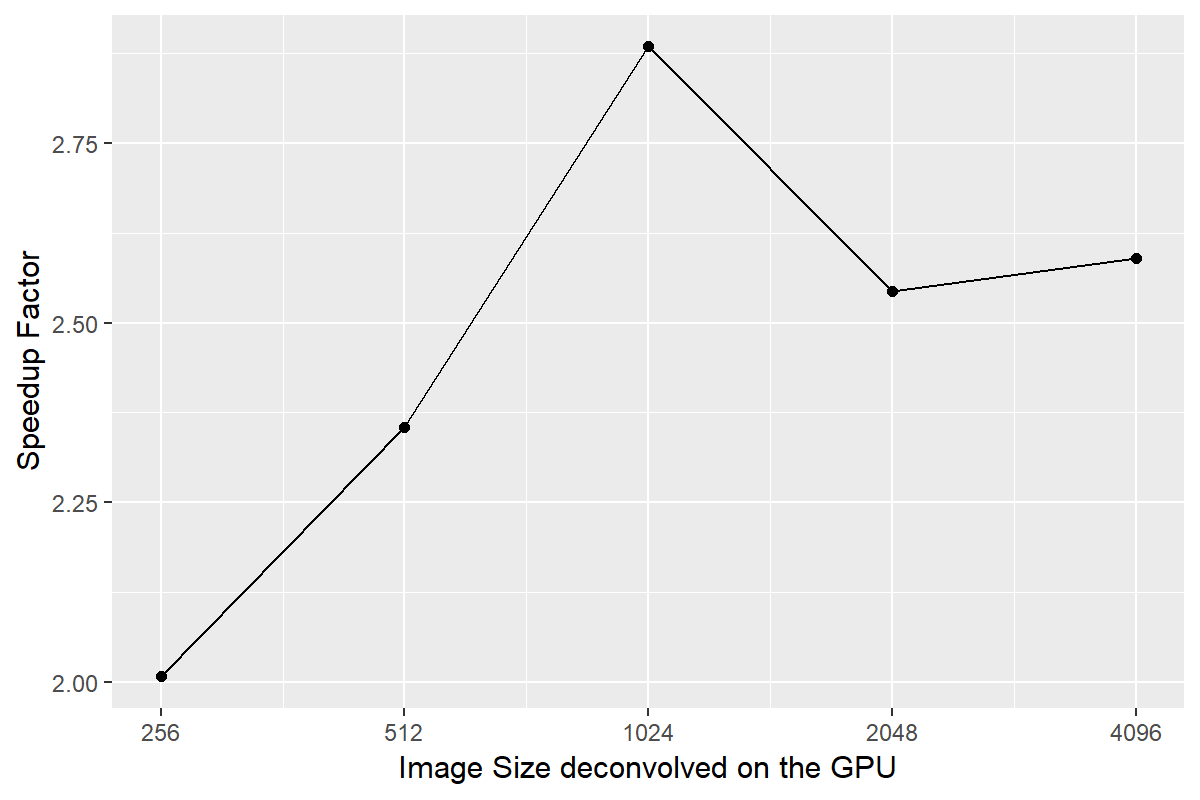
\includegraphics[width=1.00\linewidth]{./chapters/10.results/speedup/gpu.png}
	\end{subfigure}
	\caption{Speedup by using MPI or GPU acceleration}
	\label{results:speedup:figure}
\end{figure}

As we mentioned before, the speedup we achieve by using nodes/processors in MPI is the best-case scenario. As the best case scenario, we achieve a significant performance increase by using more nodes/processors. Up to 16 processors, the speedup we achieve is at least linear. Afterwards however the speedup diminishes. With 32 processors, we are only marginally faster than with 16. If the nodes would run two different physical machines, the speedup we achieve would depend mainly on the latency of the connection. 

The speedup we achieve by using GPU acceleration is fairly constant over the image size. The speedup factor varies around 2.5. Ideally, we would like to combine the distributed and the GPU implementation. However, this is not useful with the current implementation: The main bottleneck in the MPI implementation is the communication step in each iteration. 

We do not have a CLEAN implementation in our .Net Core pipeline. However, we mentioned the similarities between the serial coordinate descent and CLEAN in Section \ref{cd:similarities}. A single serial coordinate descent iteration is roughly equivalent to a standard CLEAN iteration. If we assume we need 14'000 CLEAN iterations to reconstruct an image, we can get a rough estimate by comparing the wall-clock time of 14'000 serial coordinate descent iterations. In this case, CLEAN is roughly 7 times faster than the current serial coordinate descent iteration.

Overall the serial coordinate descent algorithm with GPU acceleration is still several factors slower than CLEAN. The speedup we achieve with MPI is significant. But because serial coordinate descent and CLEAN have such a similar structure, we can expect a similar speedup with a CLEAN-MPI implementation. We need another method to speed up our deconvolution algorithm.


\subsection{Effect of approximating the $PSF$} \label{results:gradients}
Hypothesis.

As we described in Section \ref{gradients}, the $PSF$ for deconvolution is as big as the image. For wide field-of-view observations of MeerKAT, the $PSF$ is approximately a gaussian with decreasing pixel values the further we move from the center. Most of the values in the $PSF$ are close to zero. The question is, what effect has an approximate deconvolution with a smaller $PSF$? If we can approximate the deconvolution with a small enough $PSF$, we can solve patches of the image independently of each other. However, the $PSF$ approximation may need more major cycles to converge.



%We compare the objective value and see if it converges. Measure speedup

%PSF is responsible for calculating the gradient of coordinate descent.

%Remember CD:

%The two approximation methods

The effect of approximating the $PSF$ are not clear. We know that thanks to the $w$-term in the visibilities, the $PSF$ is not constant over the image. We already need several major cycles to converge. With a good approximation of the $PSF$, we may speed up the individual iterations of coordinate descent without needing more major cycle.

We presented two methods to approximating the $PSF$ for the deconvolution in Section \ref{gradients}. Method 1 updates only a fraction of the gradients, and Method 2 uses a fraction of the $PSF$ for deconvolution. We test both methods on the LMC data and explore what effects the approximations have on the reconstruction.





\subsubsection{Method 1: Approximate gradient update}
Our coordinate descent method updates the map of gradients after each iteration.  Method 1 starts with the same map of gradients as the original, but then only updates a fraction of the gradients in each iteration. It updates a rectangle of the most significant gradients.With each coordinate descent iteration, the map of gradients gets less accurate. Because we do an approximate update of gradients, this method should converge to the same result as the original with enough major cycles.

At the beginning of each major cycle, we calculate the objective value of the current solution. We compare the objective value and the wall-clock time of the original and the approximate gradient update. This is a minimization problem, meaning the lowest objective is the most accurate reconstruction (according to the elastic net regularization).

\begin{figure}[h]
	\centering
	\begin{subfigure}[b]{0.58\linewidth}
		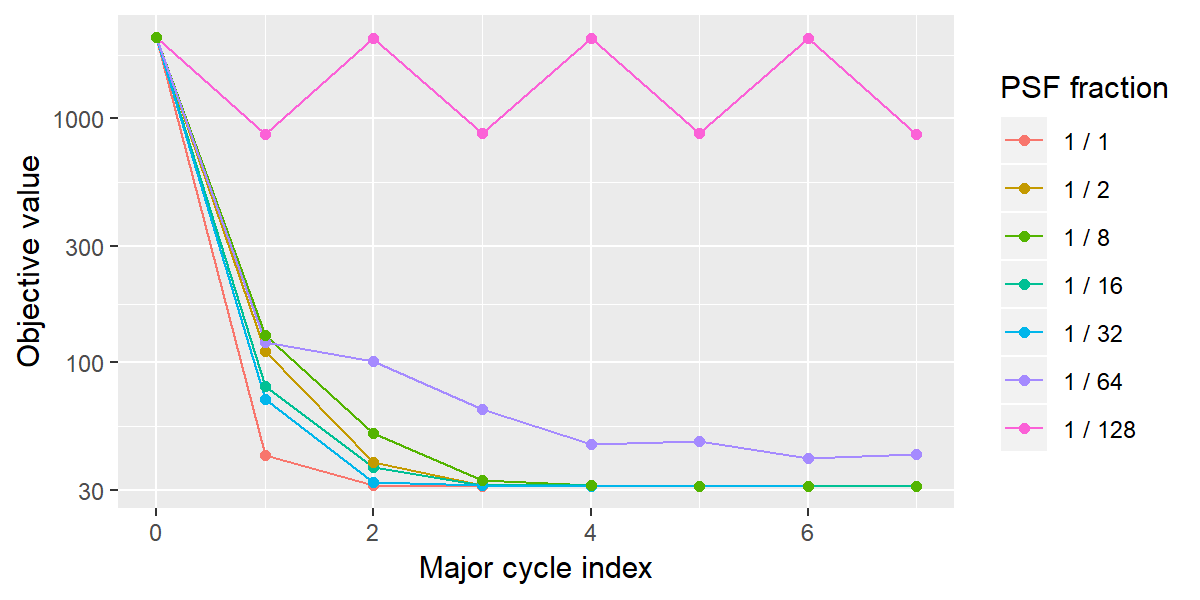
\includegraphics[width=\linewidth]{./chapters/10.results/gradient/ApproxUpdate/size.png}
	\end{subfigure}
	\begin{subfigure}[b]{0.195\linewidth}
		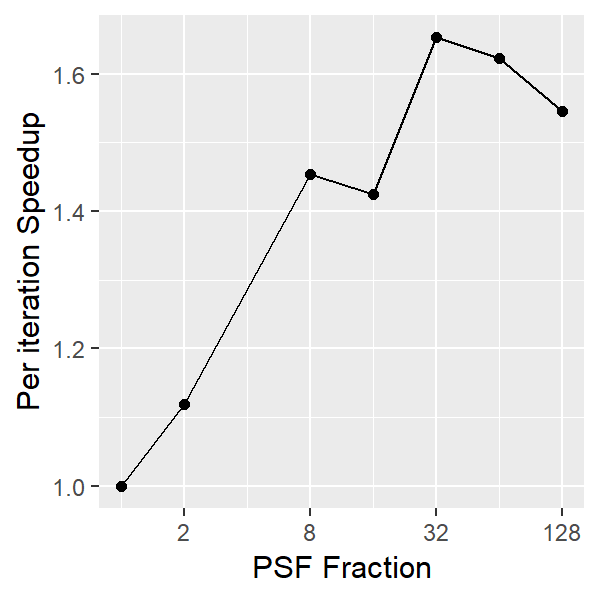
\includegraphics[width=\linewidth]{./chapters/10.results/gradient/ApproxUpdate/speedup_iter.png}
	\end{subfigure}
	\begin{subfigure}[b]{0.195\linewidth}
		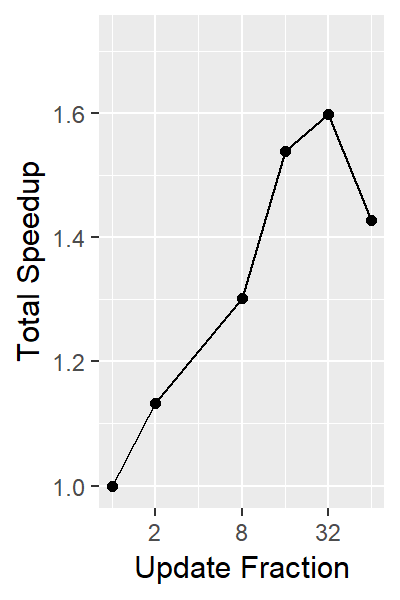
\includegraphics[width=\linewidth]{./chapters/10.results/gradient/ApproxUpdate/speedup_total.png}
	\end{subfigure}
	
	\caption{Effect of only updating a fraction of the gradients.}
	\label{results:gradients:update}
\end{figure}

The smallest fraction of gradient updater, for which coordinate still converges is $\frac{1}{64}$ of the total update. Meaning, we can update only a rectangle of $48^2$ pixels, or an image patch of 72 arc-seconds in size. However, it is obvious from the Figure \ref{results:gradients:update} that coordinate descent needs more major cycles to converge with such an extreme approximation.

With less extreme approximations, we also reduce the number of necessary major cycles. The approximation of $\frac{1}{32}$ needs two more major cycle, while all other need the one more as the original method\footnote{6 cycles to converge, and one extra cycle which is here to measure the final objective}. The objective values of the approximations end within 0.03\% of the original(the objective value of the approximations are higher by a factor of 0.0003).

Figure \ref{results:gradients:update} also shows two speedup comparisons. The speedup from the approximation is harder to quantify. For one, each iteration of coordinate descent becomes cheaper, because we only update a small part of the gradient map. This is the per iteration speedup. The second speedup Figure compares the overall time spent in deconvolution. Although each iteration becomes cheaper with the approximation, we may need more iterations to converge. Also, we have an implicit path regularization in the approximation. Therefore, a speedup per coordinate descent iteration does not necessarily lead to an overall speedup.

As we discussed in section In Section \ref{gradients:pathreg}, we have a limit in each major cycle to how far we can trust our approximation. That is why in the first major cycle coordinate descent gets started with a higher $\lambda$ regularization than specified. In each successive major cycle, we reduce the $\lambda$ parameter until we reach the specified value. This is an implicit form of path regularization, and may help speeding up the convergence rate of coordinate descent in general \cite{friedman2010regularization}. In our case, we need path regularization to ensure convergence over several major cycles (Aggressive approximations like $\frac{1}{64}$ start to oscillate over several major cycle). Notice that the overall speedup in Figure \ref{results:gradients:update} is lower than the speedup we get per iteration. This suggests path regularization as implemented here does not speed up convergence rate.

Overall with gradient update approximations give us a speedup factor of around 1.5. Depending on how aggressive we approximate, We need one or two more major cycles than the original coordinate descent deconvolutions. This puts gradient update approximations on par with multi-scale CLEAN in terms of major cycles. 

\subsubsection{Method 2: Approximate deconvolution}
In this method, we use a fraction of the total $PSF$ for deconvolution. This method solves a different deconvolution problem, where the $PSF$ is for example only $\frac{1}{8}$ the size. The downside is that method 2 is not guaranteed to converge to the same optimum. Nevertheless, we solve the approximate deconvolution problem with several different fractions of the $PSF$ and compare how close the approximate solution is to the original.

As before, we measure the true objective value for the approximate solution at the beginning of each major cycle iteration. The Figure \ref{results:gradients:aproxDeconv} compares the approximate deconvolution to the original.

\begin{figure}[h]
	\centering
	\begin{subfigure}[b]{0.58\linewidth}
		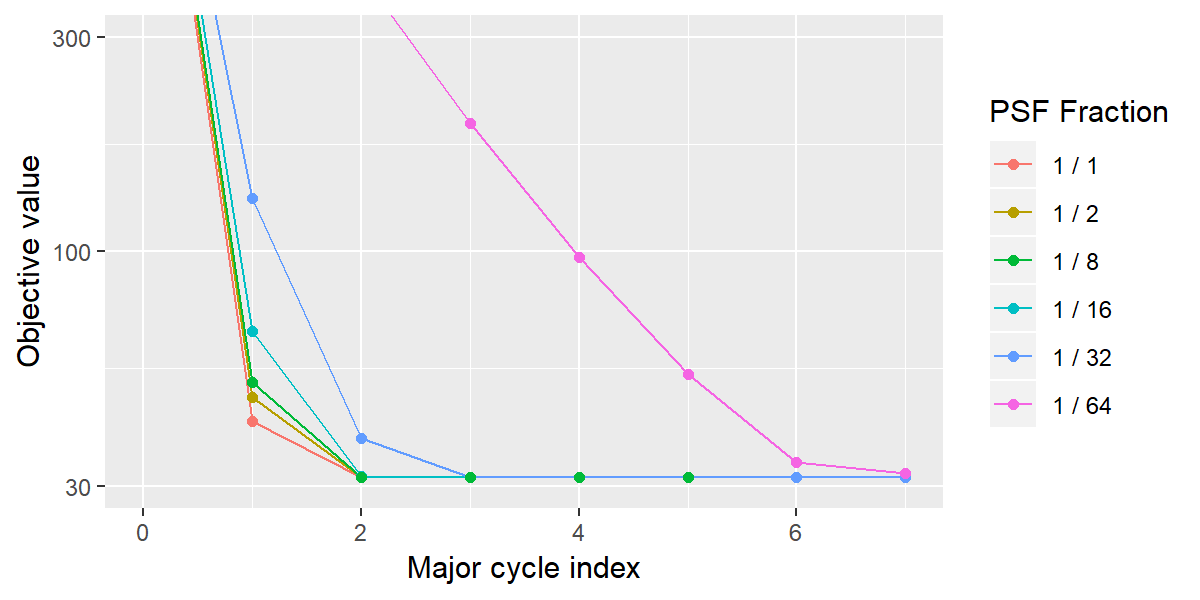
\includegraphics[width=\linewidth]{./chapters/10.results/gradient/ApproxDeconv/size.png}
	\end{subfigure}
	\begin{subfigure}[b]{0.195\linewidth}
		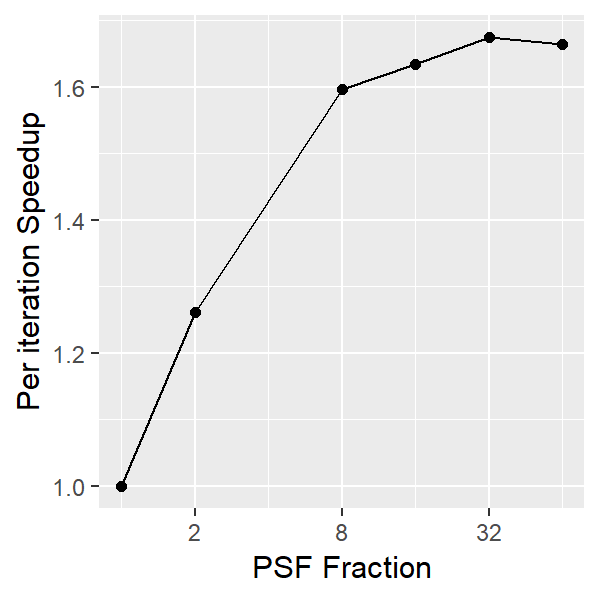
\includegraphics[width=\linewidth]{./chapters/10.results/gradient/ApproxDeconv/speedup_iter.png}
	\end{subfigure}
	\begin{subfigure}[b]{0.195\linewidth}
		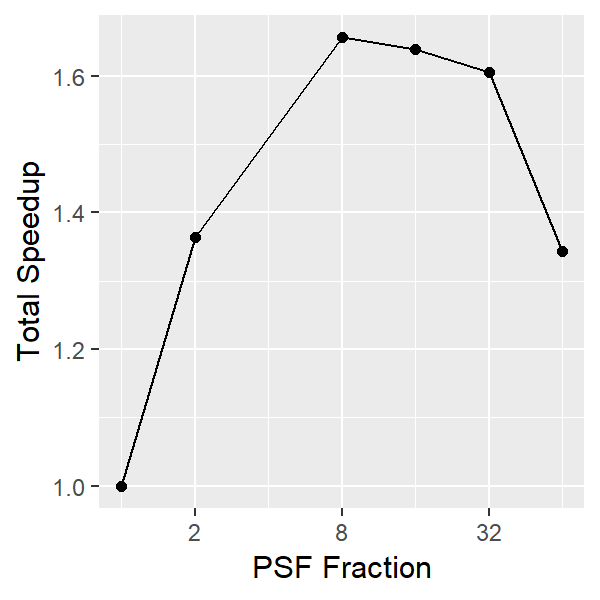
\includegraphics[width=\linewidth]{./chapters/10.results/gradient/ApproxDeconv/speedup_total.png}
	\end{subfigure}
	
	\caption{Effect of the L1 and L2 Norm separately.}
	\label{results:gradients:aproxDeconv}
\end{figure}

The performance is similar to the first method at first glance. Both methods converge in a similar manner, with a similar factor of speedup. For the $PSF$ fraction $\frac{1}{64}$ this is largely due to the same path regularization used in this method. For larger $PSF$'s, starting from $\frac{1}{16}$, the path regularization becomes less important with this method, as it only effects the regularization parameter $\lambda$ of major cycle index 0. Indeed, this method is less likely to oscillate and seems to have a more stable convergence.

The approximate deconvolution converges faster than the first method. At the start of the same major cycle, this method always has a lower objective. However, it is not guaranteed to converge to the same result. This can be seen in the fact that it never reaches the same objective value as the original. The objective value of the approximation is within 0.07\% (Factor of 0.0007, roughly twice the factor of the first method). The difference gets more significant, the more extreme we chose the deconvolution approximation.

Nevertheless, the approximate deconvolution converges surprisingly close to the original solution. The question is, is this difference of 0.07\% in the objective value significant? The answer to this question depends on what kind of error the approximation introduces in the image. The obvious error is that the approximation chronically under-estimates the pixel values: The maximum pixel value in N132D of the original is 0.0024 Jansky/beam, while the maximum of the $\frac{1}{16}$ approximation is 0.00235 Jansky/beam. The pixel magnitude is important in the self-calibration regime \cite{offringa2017optimized} (When we take the result of the reconstruction and try to improve the calibration).

The under-approximation of pixel values is an error we cannot ignore. One naive remedy is to start with the deconvolution approximation, but switch to the original $PSF$ after a certain number of major cycle. This would give us the guarantee to converge to the same result, but let us use an approximation at the start. We propose another solution: Combining the two approximation methods.


\subsubsection{Combination of Method 1 and 2}\label{results:gradients:comparison}
The two approximation methods have two different shortcomings: Approximate gradient update (method 1) converges more slowly, and converges to the same result as the original. Approximate deconvolution (method 2) converges faster than method 1, but does not converge to the same result. Here, we combine the two methods to remedy the shortcomings: For the first couple of major cycles, we use approximate deconvolution, and then switch to approximate gradient update.

We compare the original, approximate gradient update, approximate deconvolution and our combination in. We use the factor $\frac{1}{16}$ for approximations, meaning we update $\frac{1}{16}$ of the gradients, and do the approximate deconvolution with $\frac{1}{16}$ of the $PSF$.

\begin{figure}[h]
	\centering
	\begin{subfigure}[b]{0.33\linewidth}
		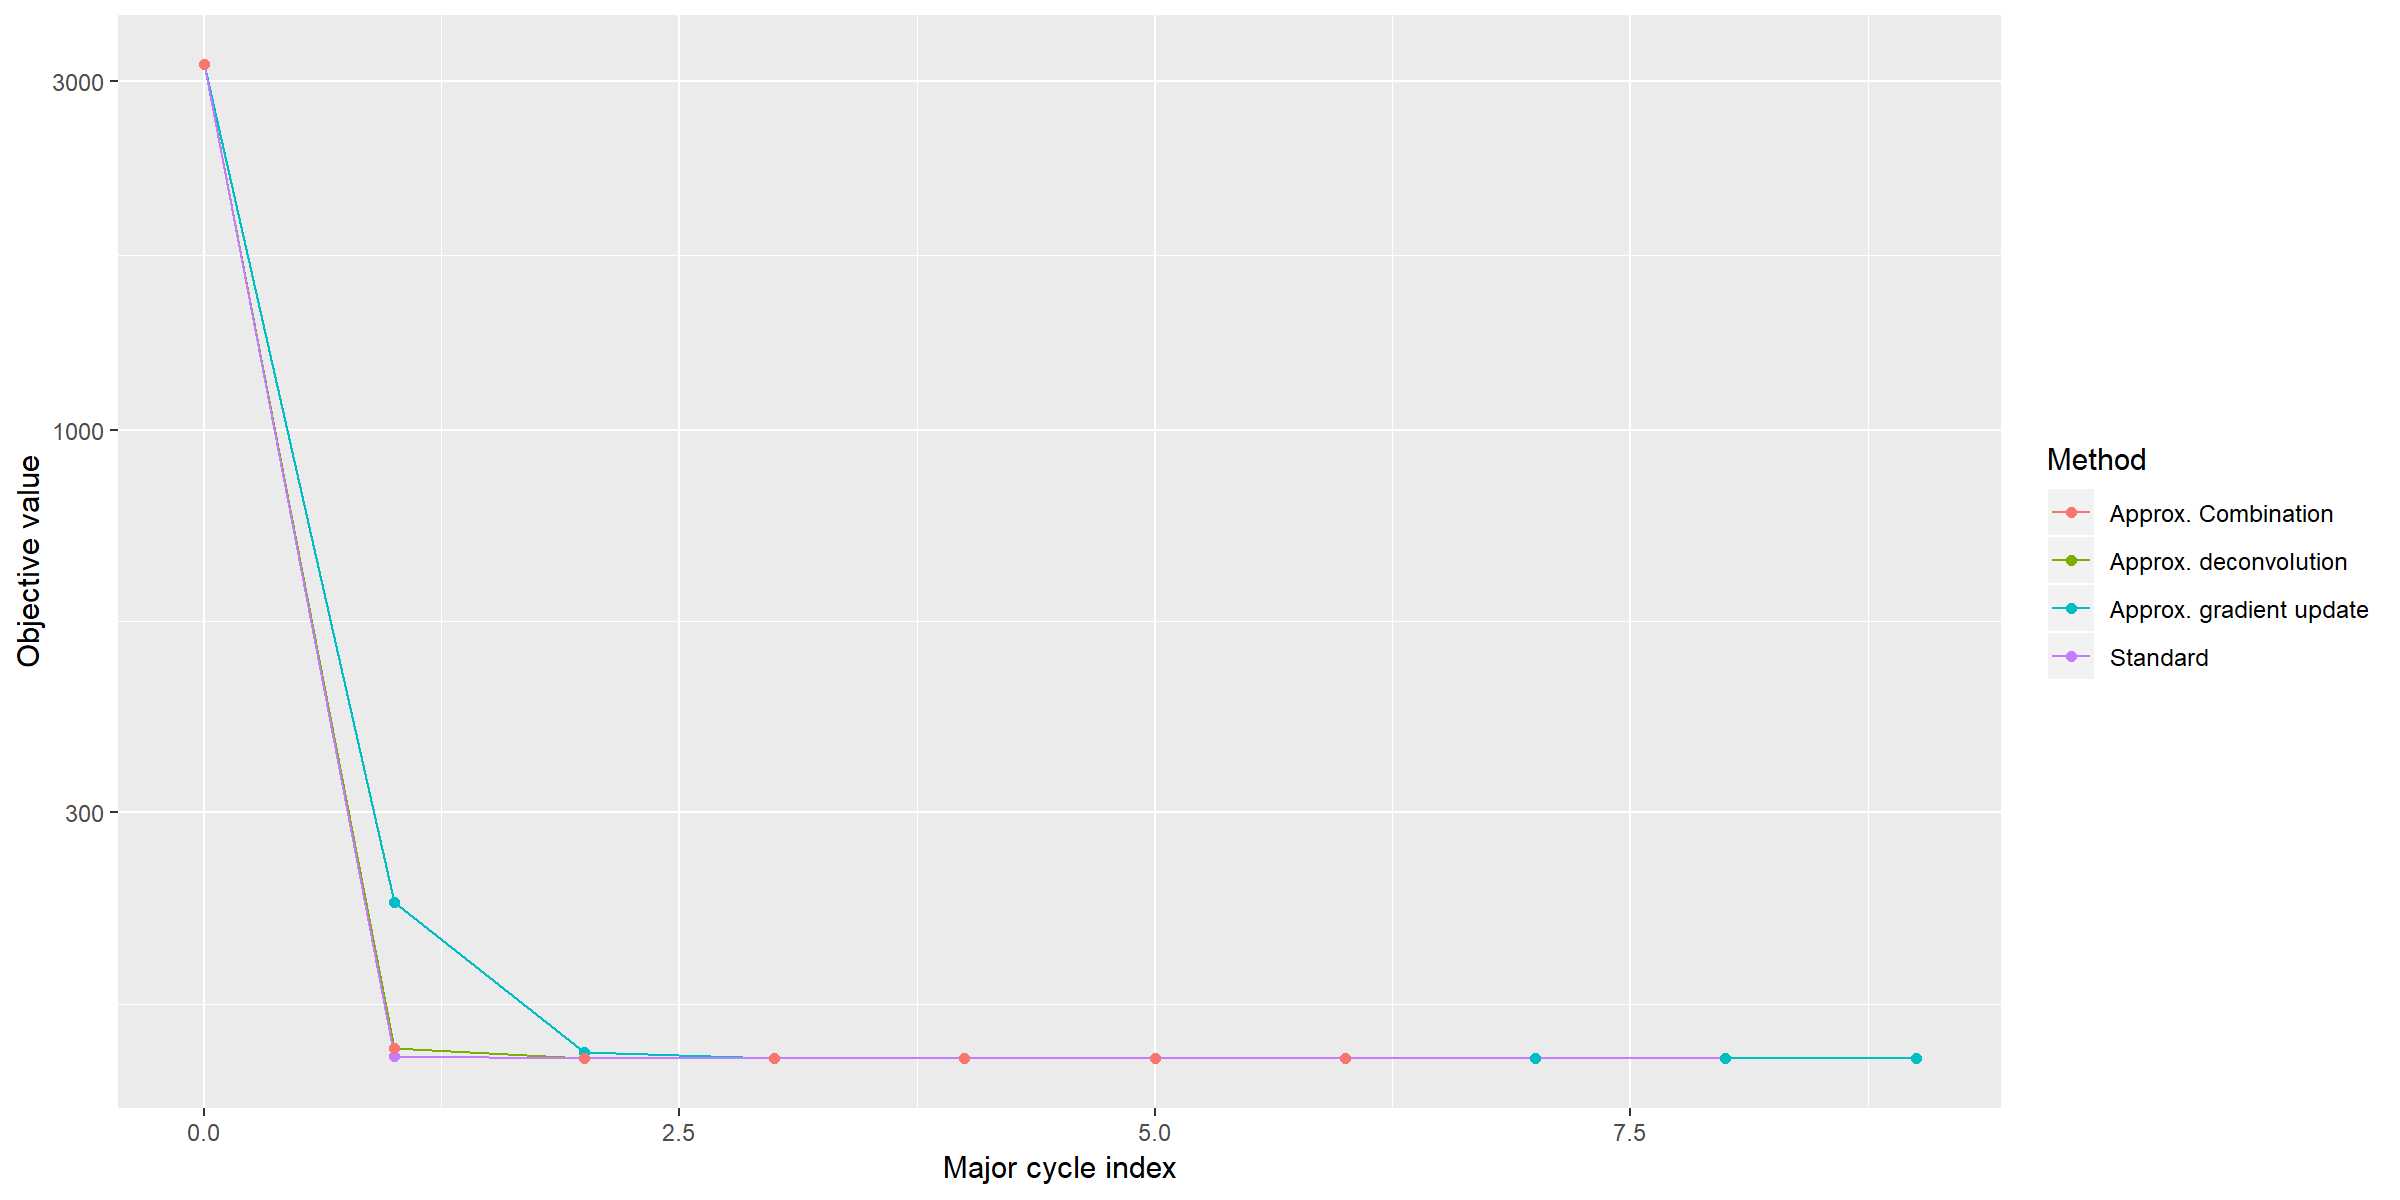
\includegraphics[width=\linewidth]{./chapters/10.results/gradient/comparison.png}
	\end{subfigure}
	\begin{subfigure}[b]{0.66\linewidth}
		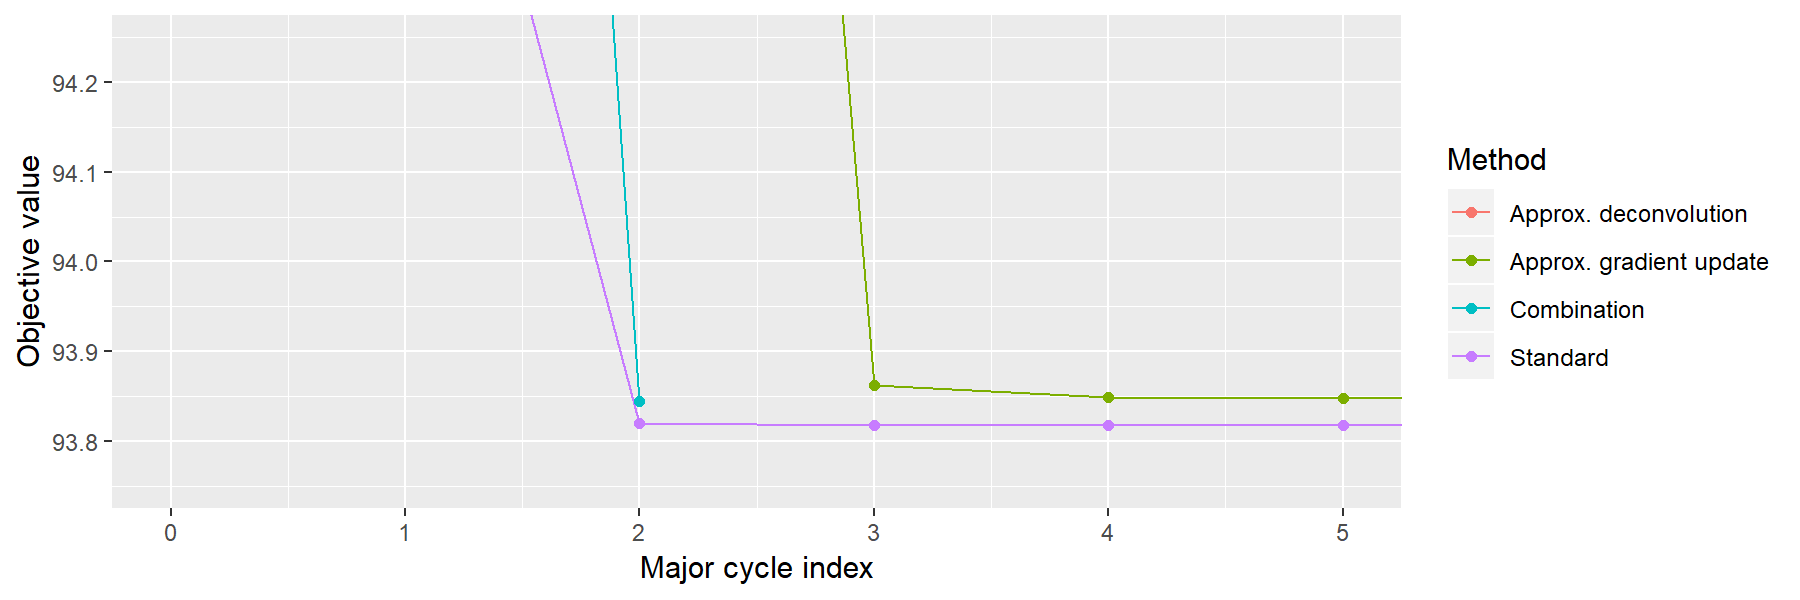
\includegraphics[width=\linewidth]{./chapters/10.results/gradient/comparison_zoom.png}
	\end{subfigure}
	
	\caption{Comparison of the two methods using the fraction $\frac{1}{16}$ of the $PSF$.}
	\label{results:gradients:comparison:figure}
\end{figure}

Figure \ref{results:gradients:comparison:figure}

We switch from approximate deconvolution to gradient update after the path regularization has reached the target $\lambda$ for the first time. In the case of the LMC data, the implementation uses approximate deconvolution for major cycle index 0 and 1, and then switches to approximate gradient update.

\begin{table}
	\centering
	\begin{tabular}{ c||c|c } 
		\hline
		Method & Iteration Speedup & Total Speedup \\ \hline \hline
		Original & 1.00 & 1.00 \\ 
		(Method 1) Approx. gradient update & 1.66 & 1.55 \\ 
		(Method 2) Approx. deconvolution & 1.67 & 1.68 \\ \hline
		Combination & 1.69 & 1.68 \\ 
		\hline
	\end{tabular}

	\caption{Results when combining the two approximation methods}
	\label{results:gradients:comparison:speedup}
	
\end{table}
Speedup. Combination is the fastest overall and leads to the lowest objective function. Actually beats the original by a small margin.
Approximation errors are not correlated. We can use Method 1 to remove the approximation errors of Method 2.


\begin{figure}[h]
	\centering
	\begin{subfigure}[b]{0.3\linewidth}
		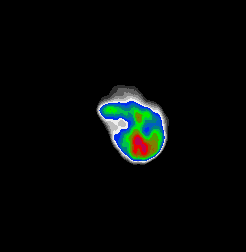
\includegraphics[width=1.00\linewidth]{./chapters/10.results/cleancomp/n132_cd.png}
		\\
		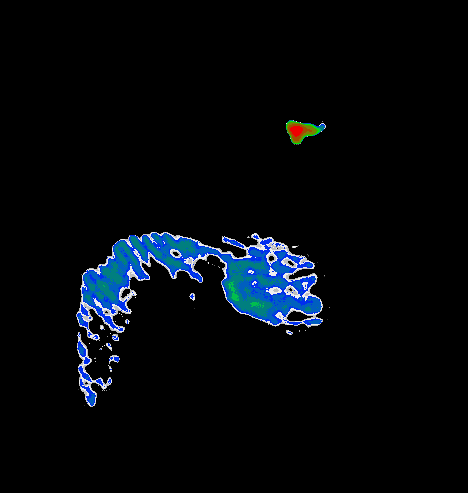
\includegraphics[width=1.00\linewidth]{./chapters/10.results/cleancomp/cd_calibration.png}
		\caption{Original CD}
	\end{subfigure}
	\begin{subfigure}[b]{0.3\linewidth}
		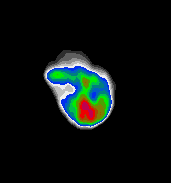
\includegraphics[width=1.00\linewidth]{./chapters/10.results/gradient/combined/combined_n132d.png}
		\\
		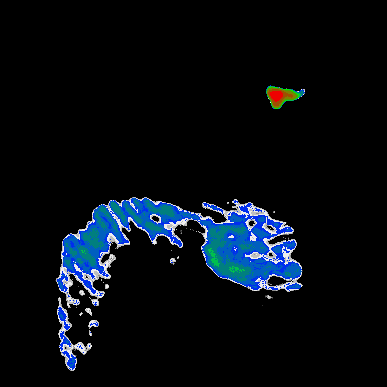
\includegraphics[width=1.00\linewidth]{./chapters/10.results/gradient/combined/combined_calibration.png}
		\caption{Combined approximation}
	\end{subfigure}

	\caption{Image comparison to approximation}
	\label{results:gradients:comparison:image}
\end{figure}

Figure \ref{results:gradients:comparison:image} compares the original result with the result of the combined approximation. Virtually identical. Same problem with calibration. Only visual difference in the extended emission with calibration errors. 


Difference is negligible. We can use the approximation and arrive at the same result. Speedup of a factor 1.6
How many major cycles: One more than the original. But same as multi-scale CLEAN.

